%%%%%%%%%%%%%%%%%%%%%%%%%%%%%%%%%%%%%%%%%
% Note:
% The \lipsum[#] commands throughout this template generate dummy text
% to fill the template out. These commands should all be removed when 
% writing assignment content.
%
%%%%%%%%%%%%%%%%%%%%%%%%%%%%%%%%%%%%%%%%%

%----------------------------------------------------------------------------------------
%	PACKAGES AND OTHER DOCUMENT CONFIGURATIONS
%----------------------------------------------------------------------------------------

\documentclass[a4]{article}

\usepackage{fancyhdr} % Required for custom headers
\usepackage{lastpage} % Required to determine the last page for the footer
\usepackage{extramarks} % Required for headers and footers
\usepackage{graphicx} % Required to insert images
\usepackage{lipsum} % Used for inserting dummy 'Lorem ipsum' text into the template
\usepackage[nottoc,numbib]{tocbibind}
\usepackage[utf8]{inputenc}
\usepackage{hyperref}
\usepackage{verbatim}

\usepackage[justification=centering]{caption}
\usepackage[norule]{footmisc}


\usepackage[francais, english]{babel}%les accents et écritures françaises frenchb, francais
\usepackage[T1]{fontenc}
 \usepackage{tikz}%c'est des packages obligatoires pour les maths, enfin je crois%
\usepackage{calc}%celui-ci est obligatoire pour certaines formules de maths%
\usepackage{animate}%les deux suivantes pour des dessins et animations, je crois%
\usepackage{plain}
\usepackage{amsmath}%maths%

%\usepackage{blindtext}
\usepackage{float}
\usepackage{lipsum}
%\usepackage[toc,page]{appendix}


% Margins
\topmargin=-0.45in
\evensidemargin=0in
\oddsidemargin=0in
\textwidth=6.5in
\textheight=9.0in
\headsep=0.25in 

\linespread{1.15} % Line spacing

% Set up the header and footer
\pagestyle{fancy}
%\lhead{Master Thesis} % Top left header
%\chead{\hmwkClass\ (\hmwkClassInstructor\ \hmwkClassTime): \hmwkTitle} % Top center header
\chead{} % Top center header
\rhead{\bfseries\leftmark} % Top right header
%%\rhead{\firstxmark} % Top right header
\lfoot{\hmwkAuthorName} % Bottom left footer
%\lfoot{\lastxmark} % Bottom left footer
\cfoot{} % Bottom center footer
\rfoot{\thepage} % Bottom right footer
\renewcommand\headrulewidth{0.4pt} % Size of the header rule
\renewcommand\footrulewidth{0.4pt} % Size of the footer rule

\setlength{\parindent}{2em}
\setlength{\parskip}{1em}

\renewcommand\contentsname{Table des matières}
\renewcommand\refname{Bibliographie}

\newcommand{\hmwkTitle}{Generating Synthetic Mobility Trajectories\\By Applying Machine Learning} % Assignment title
\newcommand{\hmwkFinalDate}{January 2018} % Due date
\newcommand{\hmwkClass}{Master of Science in Information Systems} % Course/class
\newcommand{\hmwkClassTime}{08:30} % Class/lecture time
\newcommand{\hmwkClassInstructor}{Supervised by Prof. Benoît Garbinato\\and M.Sc Vaibhav Kulkarni} % Teacher/lecturer
\newcommand{\hmwkAuthorName}{Yannick Patschke}% Your names
\newcommand{\hmwkEmail}{yannick.patschke@unil.ch}% Your names


\newcommand\blankpage{%
    \null
    \thispagestyle{empty}%
    \addtocounter{page}{-1}%
    \newpage}


\newcommand*{\captionsource}[2]{%
  \caption[{#1}]{%
    #1%
    \\\hspace{\linewidth}%
    \textbf{Source:} #2%
  }%
}

%----------------------------------------------------------------------------------------
%    TITLE PAGE
%----------------------------------------------------------------------------------------

\title{
\begin{figure}[H]
    \centering

\includegraphics[width=6cm]{unil.pdf}
\end{figure}
%\vspace{.5in}
\textmd{\hmwkClass}\\
\vspace{0.5in}
\textmd{\textbf{\hmwkTitle}}\\
\vspace{0.5in}
%\author{\textbf{\hmwkAuthorName}}
\textmd{\textbf{By \\ \hmwkAuthorName}}\\
\vspace{0.5in}\large{\textit{\hmwkClassInstructor\ }}
\date{\hmwkFinalDate}
}

%----------------------------------------------------------------------------------------
\setlength\parindent{0pt} % no indentation

\begin{document}

\maketitle
\thispagestyle{empty}
\addtocounter{page}{-1}


%----------------------------------------------------------------------------------------
%    Empty Page
%----------------------------------------------------------------------------------------

\clearpage % end title page
\begingroup
  %\pagestyle{empty}
  \null
  \newpage
\endgroup


%----------------------------------------------------------------------------------------
%    Abstract Page
%----------------------------------------------------------------------------------------
\newpage
\begin{abstract}
%Learning mobility behaviors of users by applying M L
The purpose of this master thesis is to capture accurate human mobility behavior, in order to generate realistic synthetic mobility trajectories. An increasing number of applications have appeared about mobility data, but unfortunately, they are still restraint mainly due to the need for large datasets and the sharing privacy restrictions of user data.
%existing works
Many mathematical models already exist to generate trajectories by using (random) stochastic processes to create trajectories, but none of them clearly succeeded in capturing a realistic human behavior.
%What we do ML, Memory, 3 parts
Therefore we choose to use machine learning models to extract information on human trajectories, in order to improve results by adopting a methodology of mobility prediction and optimization.
% predictions
Among four models used, the Recurrent Neural Network (RNN) can capture long-term time dependency and seems to perform better. The predicted trajectories with this model recall real trajectories.
%optimization
We fine-tune the model by selecting appropriate hyperparameters.
% generation
Finally, we focused on generating trajectories by creating and comparing three different generators; one based on random, one based on best probability and the last one on random choice probability. According to well-defined metrics, we found that the Random Choice Probability Generator performs better to generate realistic human trajectories.
%General conclusion
Although this technique provides satisfactory results, such models can be improved by capturing the true distribution of human mobility.
\end{abstract}


%----------------------------------------------------------------------------------------
%    TABLE OF CONTENTS
%----------------------------------------------------------------------------------------

\newpage
\tableofcontents



%----------------------------------------------------------------------------------------
%    Acknowledgements
%----------------------------------------------------------------------------------------
\newpage
\setcounter{secnumdepth}{0}
\section{Acknowledgements}
%\addcontentsline{toc}{section}{Acknowledgements}
\thispagestyle{empty}

%\topskip0pt
%\vspace*{3.5in}
I would like to thank Vaibhav Kulkarni for all the help provided during this project. Many thanks also to Prof. Benoît Garbinato and all the team of the Distributed Object Programming Lab for their warm welcome during this last semester. 

I would also like to express my thanks to Lucien Krapp for all our useful discussions and the access to his server. 

Finally, I wish to thank my mother for her support and encouragement throughout all my studies.
%\clearpage
\setcounter{secnumdepth}{1}

%----------------------------------------------------------------------------------------
%    Introduction
%----------------------------------------------------------------------------------------
\newpage
\section{Introduction}
%context (problems)
There are several useful applications where mobility data can be integrated, such as traffic management, urban planning, and consumer profiling. However, these applications are struggling to exist mainly due to the need for large datasets and privacy restrictions of user data. It is why we focused on generating synthetic mobility trajectory by capturing human mobility behavior. For now, in practice, it is still difficult to generate trajectories of people due to the complex behaviors that people exhibit. Generating trajectories of projectiles has already been done with ballistic and even more complex trajectories such as fluid dynamics can be done with a known accuracy. However, generating trajectories for living entities becomes difficult. For instance, with insects, ants colonies are still studied to understand their behavior within a colony and to create better algorithms to solve the traveling salesman problem. Indeed many mathematical models exist to describe or generate trajectories for different purposes, such as birds migration, predators behavior, and human mobility. They used (random) stochastic process to create trajectories, but none of them clearly succeeded in capturing a realistic human behavior. The main issues with these models are their huge boundaries or too random behavior. So capturing real human behaviors and generating their trajectories is still a challenge.

%approach
We choose to use machine learning models to extract information on real human trajectories. Unlike the Markov processes, we focused on the idea that having some memory of past positions can be used to predict the following positions of a person. As movements of people go clearly often into one specific direction, it is interesting to know what were their last steps in order to better predict or generate their trajectories. It is why capturing human mobility behaviors will be possible only if we can integrate some part of their movement. Furthermore, we simplified the problem by using areas of interest where people stay more time instead of geographical coordinates. The project was divided into three parts: Prediction, Optimization, and Generation. 
%prediction
The first part consists in comparing the performances to predict the next places of people of different machine learning models: Linear Regression, Logistic Regression, Neural Network (NN) and the Recurrent Neural Network - Long Short-term Memory (RNN-LSTM). These models were put in competition to predict the next positions of people based on their last position(s). Among all these models the RNN-LSTM model seems more appropriate for the task \cite{kulkarni}. Its characteristics allow it to perform great where long-term dependencies are important. Even with very basic parameters, it obtains good results. 
%optimization
Thereafter the second part tried to fine-tune the RNN-LSTM by searching for the optimal hyperparameters, in order to optimize the performances of the model. According to our tests, the maximum performances were reached with 5 timesteps and 5 hidden layers with 50 neurons each. Indeed the trajectories predicted seem more realistic. Moreover, some measures extracted from them and compared with real trajectories confirm it: the Mean, Median, Standard Deviation, and P-value are on average clearly in favor of these parameters.
%generation
During the last phase, in order to generate different successive positions, we created three different generators; Random Generator, Best Probability Generator and Random Choice Probability Generator. The first one is based only on random, while the two others are based on the RNN-LSTM model trained before. The three results were compared; the Random Generator generates no realistic human trajectories. The other two perform well with few generate steps, but the Random Choice Probability Generator is better when generating long trajectories. Moreover, many measures confirm it on generated trajectories, such as Mean, Median, Unique, Standard Deviation, and Skew.

%conclusion
Different machine learning models can be adapted in a way or another to our project. However, the importance of long-term dependencies is confirmed. It is why RNN models are predisposed to the task. Although none of these generators are yet prepared to be used in final applications, we have proved that generating synthetic mobility trajectories by learning the human mobility behavior through machine learning is possible. Moreover, such models can be improved by capturing the true distribution of human mobility.

%----------------------------------------------------------------------------------------
%    Motivation
%----------------------------------------------------------------------------------------
\newpage
\section{Motivation}%1/2
%usefull
The movements keep increasing in many fields; human, material and information. Indeed the number of shiftings, transitions, and movements in our society has never been so high and continues to increase. For more than a century, we have not stopped seeing advances in many fields; mechanics, medical, computer science and many other sciences. Every time, these advances are reserved for a small number of people, but rapidly popularized and accessible to all. We can think of the first cars rapidly popularized with the \textit{Ford T} by the brilliant \textit{Henry Ford}.
Especially since globalization, all new things have become even more rapidly accessible to the general public. Many things that were one century ago reserved for rich or a particular sector, for instance, travel, are now common and widely widespread. Our technology and also our way of life, nowadays have particularly influenced movements in our society. They have really increased and promoted the rise of movements of people, and materials. It is really difficult to imagine the amount of data that we could collect just about daily movements of goods in a city, the number of letter ships or people moving to work. Now that some technologies like the GPS and connected device are so widely used and accessible, getting all these information about movements is possible at a technological level. All this different data about mobility can be useful in some ways. Thinking only about human mobility, we can already find a lot of fields where this data could be useful \cite{kulkarni}: 
\begin{description}
  \item [Traffic management:] We could analyze the movement of people to better know the most affected areas. We could think of a way to improve the fluidity or prevent traffic jam.
  \item [Urban planning:] With the behavior of movement of people, we could predict the best areas to construct. We could increase existing area level for instance where construct a new mall to be accessible to as many people as possible.
  \item [Consumer profiling:] We could try to learn behaviors of consumers to better understand their needs or find a better way to reach them.
\end{description}
%mobility datasets difficult to obtain
The main problem is the need of a lot of data to obtain results which could make sense. It is not sufficient just to go and ask 100 people to give us their mobility data. As said before at a technological level we could obtain nearly all this data, but in practice, we are stopped by the amount of data. It is really difficult for somebody, a city, or an organization to obtain enough data in a field like mobility. Indeed, you have to ask people directly, which means to really ask a lot of people.

The second main problem will result from the free will of people and their privacy. Not a lot of people will agree to give freely their mobility data. There will always be this barrier of privacy. Rare are those who accept to give all their movements in life. Thinking of paying people to give us their traffic data is just not imaginable. If it was the case, more people would maybe participate, but the city or the organizations would need really a lot of funds. Fortunately, we live in a free country based on democracy, so trying to force people to give us the data or even find a way to collect their data without their agreement it also not possible. Based on all the above reasons, generating synthetic geospatial trajectories could be an interesting thing. Indeed it would allow us to need really a lot less data, which would mean also a lot fewer problems about collecting them.


%----------------------------------------------------------------------------------------
%    Background
%----------------------------------------------------------------------------------------
\newpage
\section{Background}% 6,7
There are already some helpful knowledge and tools really useful for our project. This section shows some of them with their respective overview and their explanations. For instance, it focuses on a machine learning overview and some of its specific models related to our work. This section speaks also about some really interesting and relevant library existing or even the dataset used.

\subsection{Machine Learning}
Nowadays Machine learning is really widespread even if most people don't really know its utility and its possibilities. Machine learning is basically to teach the machine to act in situations that differ from what we have trained it. It is a process that first begins with a training phase where the machine trains with examples. Then the next phase is an evaluating process. Indeed we give the machine new but similar data and we look at how it processes it. Which means the machine tries to work on new data based on what it has learned previously with its trained data. Without going into details, nowadays we distinguish two major types of machine learning; supervised and unsupervised.

\textbf{Supervised machine learning:} The method allows us to train the machine on example data and its results. Basically, during supervised machine learning, we show the machine examples and their correct results several times. Until the machine has learned some patterns about the data and understood that if we give it an input \textit{A} the correct answer will be \textit{B}. For instance, we can make a connection with how a human kid learns to read. The kid will try to read some simple books several times until he correctly reads and articulates all words of these books. When he has correctly read all these books, we can assume that he understands how to read different words. Therefore we can assume that if we give him another book, he will manage to read this new book even if it is the first time. For the machine, it is similar; each time the machine sees the data example, it will try to remember what it has done good or bad. Then it will try to make better the next time. So we can say that supervised machine learning, mainly uses to understand the way to go from a point \textit{A} (input data) to a point \textit{B} (output data, the correct answer).

\textbf{Unsupervised machine learning:} This method works differently; this time the machine will just train on examples without feedback of what is true or false. It means without correct answers from the example data. Imagine again a child who is given a pile of marble to tidy up separately, but with no instruction about criteria to separate them. Maybe the child will separate them by color, size, weights or others, maybe mixed criteria. He will try to find a way; the machine does the same. The machine will, for example, try to identify some attributes about the data that are similar to some examples. It will try to find a way to group them together. Here it was an example of clustering. We can see that unsupervised machine learning works more to find some structure in the data given.

In our society, we can find traces of machine learning nearly everywhere and many times. For instance in our emails with the spam classification, with some social network with facial detection on pictures, with speech recognition for example from Siri of Apple, and so many other examples can be found. Moreover, machine learning will surely continue to extend in our society. Indeed these last decades have allowed really to see the power of computer increase. Now it allows processing a large amount of data faster than before. It makes it more interesting to use machine learning; indeed machine learning needs often to work with a large amount of train data to be efficient. These last years have been really good for this field. We have seen more and more people using machine learning, not only in big organizations but also private people. 

Now everybody does not need to have an expensive computer to make machine learning, but most of the personal computers can handle machine learning in a great way. Moreover, a lot of courses have been created on the subject and a lot of services help us on machine learning, for instance: Tensorflow, Keras, Caffe, Torch, PyTorch, MXNet and others \cite{varangaonkar}. Now we can find easily what we need to work with machine learning. Some models are basic and well known while others are more complex. Now let's speak of some models that seem obvious, interesting or even promising: the Linear Regression Model, the Logistic Regression Model, the Neural Network Model, the Recurrent Neural Network and its special case with Long Short-term Memory. 

\subsubsection{Linear Regression}
\begin{figure}[t!]
\centering
\begin{minipage}{0.48\textwidth}
\centering
\raisebox{-\height}{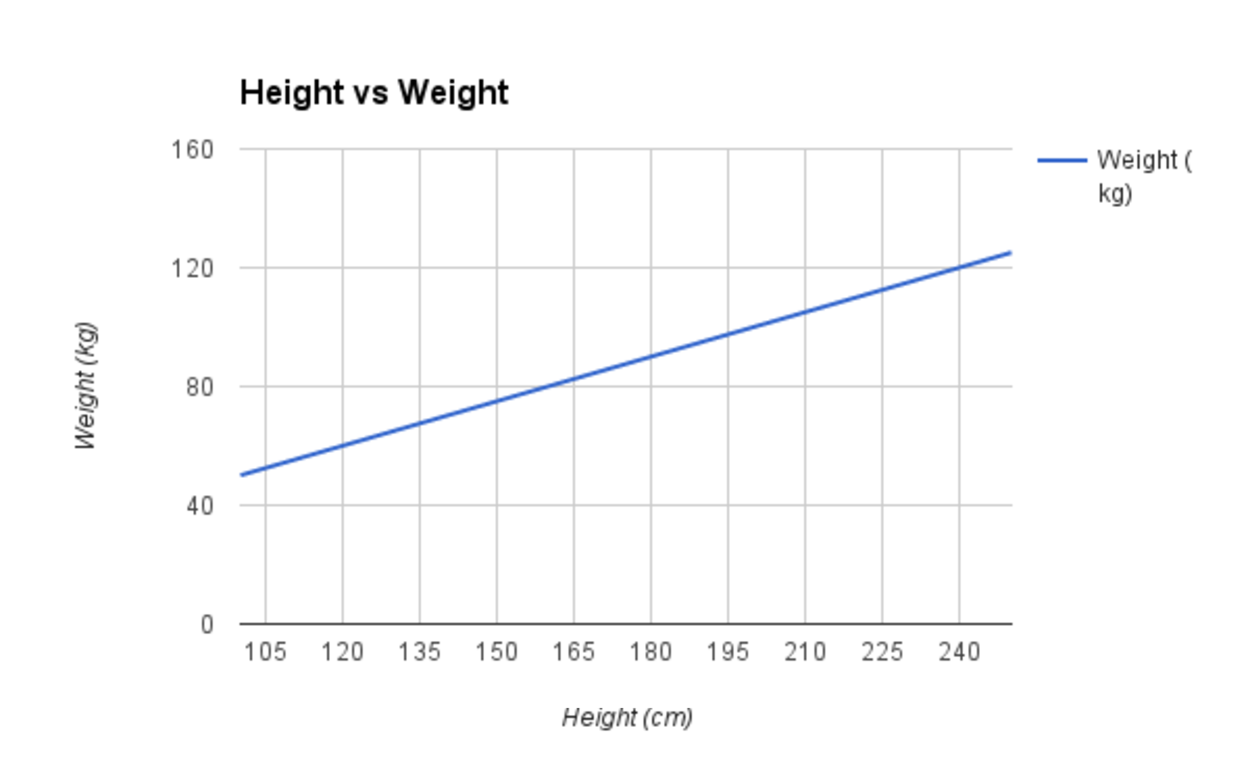
\includegraphics[width=1.05\textwidth]{LinearRegression.pdf}}
\textbf{\caption{Sample of Linear Regression - Height vs Weight \cite{brownlee2}}
\label{fig:linear1}}
\end{minipage}
\hfill
\begin{minipage}{0.48\textwidth}
\centering
\raisebox{-\height}{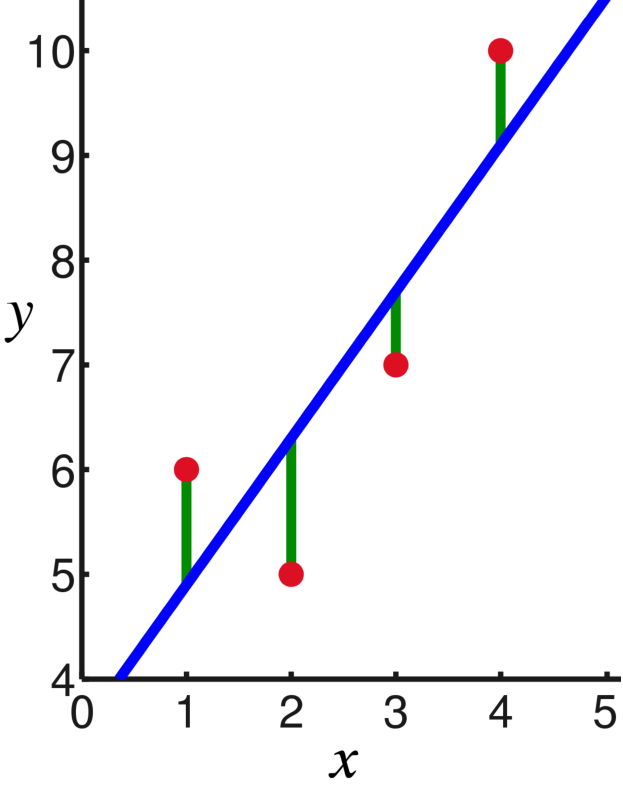
\includegraphics[width=0.5\textwidth]{LinearLeastSquares.pdf}}
\textbf{\caption{Distance to square of a Linear Regression \cite{wikipedia}}
\label{fig:linear2}}
\end{minipage}
\end{figure}
The linear regression model is clearly the most known model in statistics and machine learning. It’s generally the first model that people begin to test in order to learn basic stuff in machine learning. A linear regression model is basically a model which assumes a linear relationship \textit{(See figure: \ref{fig:linear1})} between the input variables and the output variables. The output can be calculated from a linear combination of the input variables. The representation mathematic for a simple model is $y = B0 + B1\times x$. Where $x$ represents the input, $y$ the output, $BO$ and $B1$ coefficients.
With a linear regression model, we basically try to estimate the values of its coefficients used in the equation with the data that is available. We use usually the Ordinary Least Squares procedure to minimize the sum of the squared residuals. This means that given a regression line through the data we calculate the distance from each data point to the regression line \textit{(See figure: \ref{fig:linear2})}. Then we square distances, and sum all of them. This sum is what we try to minimize. In machine learning, this sum is often called the cost function. 

During the learning phase, we optimize the values of the coefficients by iteratively minimizing the error of the model on our training data. This operation is called Gradient Descent and works by starting normally with random or zero values for each coefficient. The sum of the squared errors is calculated for each pair of input and output values. The coefficients are updated in order to minimize the errors. A learning rate is also used as a scale factor which determines the update level of the coefficients. The process is repeated until a minimum sum of squared errors seems to be obtained. At that moment, we can say that the model has converged. Then we use the model with the coefficient updated and test it on test data and train data to see how it performs. In order to evaluate its performance, we can compare training and test accuracy of the model or even the cost function from the training part and from the test part. \textit{(See \cite{brownlee2} for more details)}

\subsubsection{Logistic Regression}
\begin{figure}[t!]
\centering
\begin{minipage}{0.48\textwidth}
\centering
{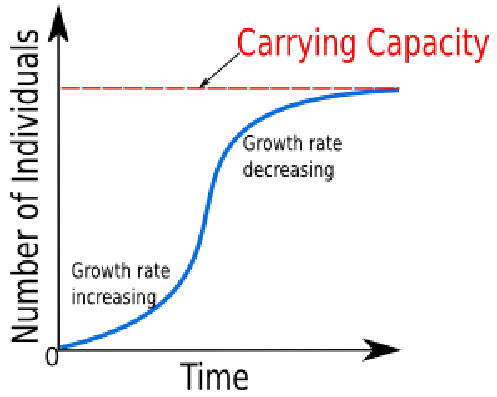
\includegraphics[width=0.75\columnwidth]{LogisticGrowthPopulation.pdf} }
\textbf{\caption{Logistic Population Growth \cite{angela}}
\label{fig:logistic}}
\end{minipage}
\hfill
\begin{minipage}{0.48\textwidth}
\centering
\raisebox{-\height}{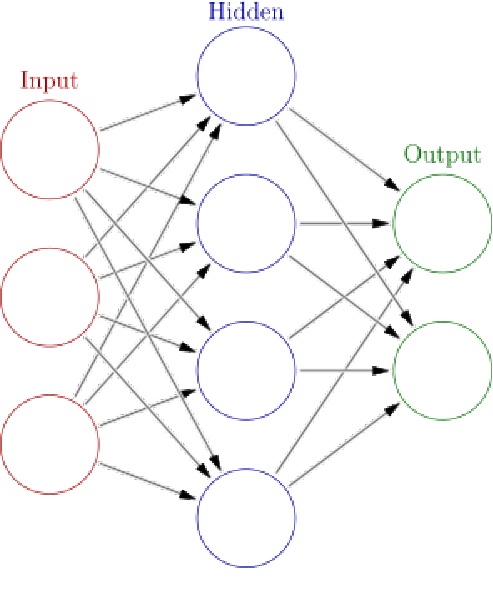
\includegraphics[width=0.61\textwidth]{NeuralNetwork.pdf}}
\textbf{\caption{Sample of a Neural Network (with 3 features, 4 neurons on one hidden layer and 2 results possible \cite{wikipedia2}}
\label{fig:nn1}}
\end{minipage}
\end{figure}
The Logistic Regression model is similar to the previous Linear Regression Model. It is also one of the most famous models. It is based mainly on the logistic function, also called the sigmoid function $1 / (1 + e^{-value})$. This function was named by \textit{Pierre François Verhulst}, who first used it to represent the population growth, where the first stage of growth is exponential, then the growth slows, and finally stops \textit{(See figure: \ref{fig:logistic})}.

The function in our case can be represented as this $y = e^{(b0 + b1*x)} / (1 + e^{(b0 + b1*x)}) $. Where $y$ is the predicted output, $b0$ is the bias and $b1$ is the coefficient for the input value. Each feature of our input data has a coefficient that we need to determine with the training step as explained before for the linear regression model. In this case, we also try to optimize the cost function at each iteration and update the coefficients values. \textit{(See \cite{brownlee3} for more details about the model)}

\subsubsection{Neural Network}
The Neural Network model is quite different. It is a more complex model and really an interesting one. The basic idea behind a Neural Network (NN) is to simulate interconnected brain cells inside a computer. We can get the machine to learn things, recognize patterns, and make decisions in a humanlike way. Moreover, you don't have to program the NN to learn explicit things: it can learn by itself, like a brain! The Neural Network can be composed of many cells that simulate the brain. The Neural Network is normally separated into three different parts \textit{(See figure: \ref{fig:nn1})}: 
\begin{enumerate}
\item Input layer: It contains input cells which are regrouped in one side of the network. These cells represent information from the outside world that the network will attempt to assimilate. It is basically all features and information that we want to learn about.
\item Output layer: It contains output cells which are on the opposite side of the network compared to those from the input layer. These cells can represent how the Neural Network responds to the information it has learned. We can see them as the result provided by the network after the data has gone throughout all of it. 
\item Hidden layer(s): It is in the middle of the network. It can be composed of one or more layers which can each of them have a various number of cells usually called neurons. These layer(s) and neuron(s) form the big part of the artificial brain. They actually influence directly the size and complexity of the network. For instance, a Neural Network with a large number of hidden layers and neurons compared to one with only one hidden layer and one neuron could, in theory, learn more complex things. It is as if we were comparing a human brain with the one of a mouse. Sadly in practice with machine learning, we can have some surprises. A small network could sometimes be better on complex data and in contrary, a complex network can be good for simple things. Indeed other parameters can influence the performance of the network on the data. 
\end{enumerate}
\begin{figure}[t!]
\centering
\begin{minipage}{0.48\textwidth}
\centering
\raisebox{-\height}{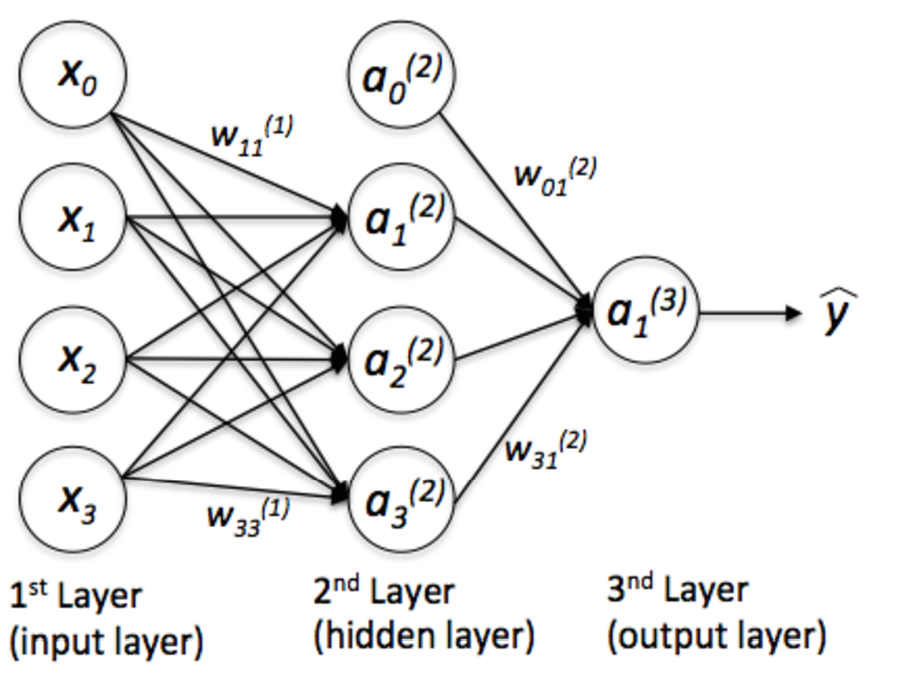
\includegraphics[width=0.77\textwidth]{NeuralNetworkWithWeight.pdf}}
\textbf{\caption{A Neural Network with weights \cite{raschka}}
\label{fig:nn2}}
\end{minipage}
\hfill
\begin{minipage}{0.48\textwidth}
\centering
\raisebox{-\height}{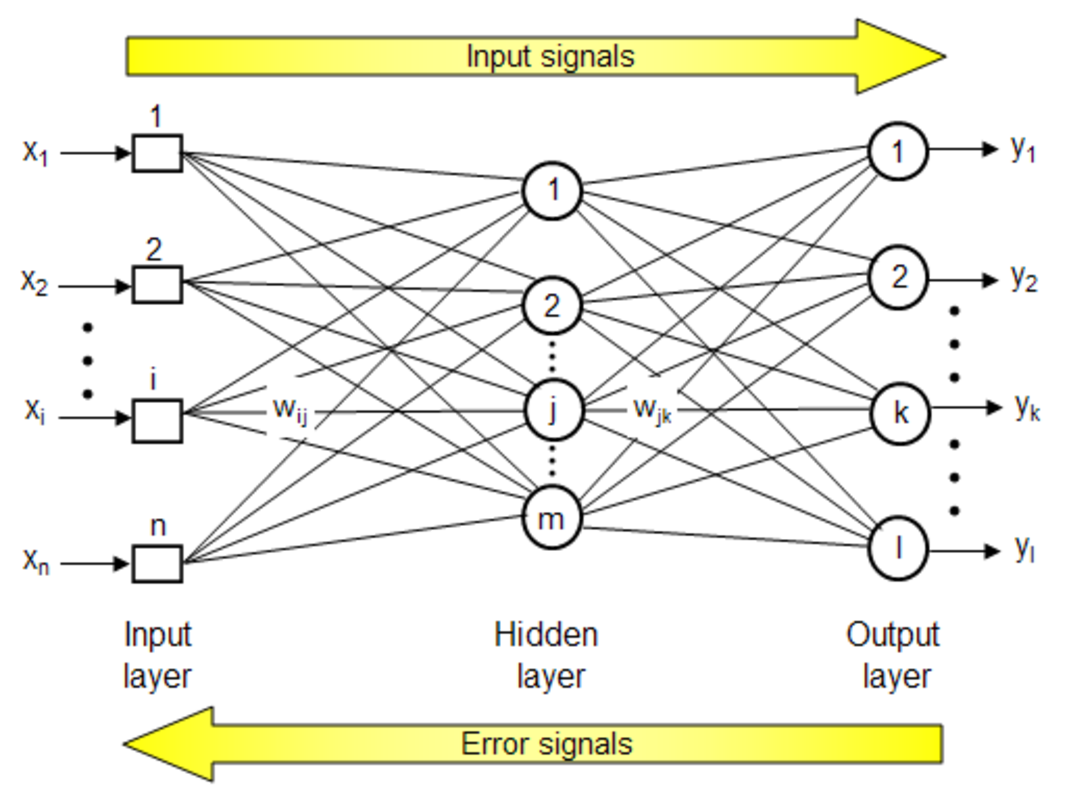
\includegraphics[width=0.85\textwidth]{NeuralNetworkWithForward.pdf}}
\textbf{\caption{A Neural Network with feed forward and back propagation \cite{buranajun2007prediction}}
\label{fig:nn3}}
\end{minipage}
\end{figure}
The connections between one cell and another are represented by a number called a weight \textit{(See figure: \ref{fig:nn2})}. Weights represent the influence that one unit has on another. More the weights are high, more the selected cell influences the cell linked.
The Neural Network as the two last models learns iteratively. We give it the training data a certain number of times and it will each time go through the entire network. Each time data goes through the network, two steps occur. The first one is a basic method called feedforward or input signals \textit{(See figure: \ref{fig:nn3})}. On this step, each unit receives inputs from the units on the left on which they are linked, and the inputs are multiplied by the weights of the connections in which their inputs go through. Every cell adds all the inputs it receives, computes some score and calls the next units it is connected to in order to give its results. The second step is where the backpropagation process occurs. It is a feedback process, in order to compare the output produced with the real output: The NN uses the difference between them to modify the weights of the connections between the cells in the NN in order to be nearest to the good results the next time. \textit{(See \cite{woodford} for more details about the model)}

To summarize, during a simple cycle, the data goes through the network by passing through the corresponding cells and links. Then the model computes scores based on the information received and weight from the connections of its cells. Thereafter the model compares results that are given and the real results in order to correct itself (its weights). The purpose is to try to perform better the next time that we give it data. Therefore this process is repeated a lot of times until it seems no longer able to improve.

\subsubsection{Recurrent Neural Network}
The Recurrent Neural Network (RNN) model works like an extension of a simple NN. RNN is similar to the NN while learning, except that it can learn and capture long-term dependencies when we need to have some persistence of some past information. Indeed when we need to work with previous events, previous results found, previous data to work on the next one, it’s where a Recurrent Neural Network becomes really useful. For instance, if we set a simple Neural Network and try to teach it to identify the nouns in a sentence by giving it only a word as input, it won't be able to perform well. Indeed a lot of information about the word given is in its context. The only way to really capture and determine this information is by looking at its context, its sentences, which means words next to it. Therefore we need to look at the entire sequences or at least a part of it. We can see an RNN as multiple copies of the same Neural Network \textit{(See figure: \ref{fig:rnn1})}. These multiple copies of networks are linked one by one and each of them passing a message to its successor. So we have a persistence of some past events or some past results. \textit{(See \cite{karpathy2016unreasonable} for more details about the model)}
\begin{figure}[t!]
\centering
{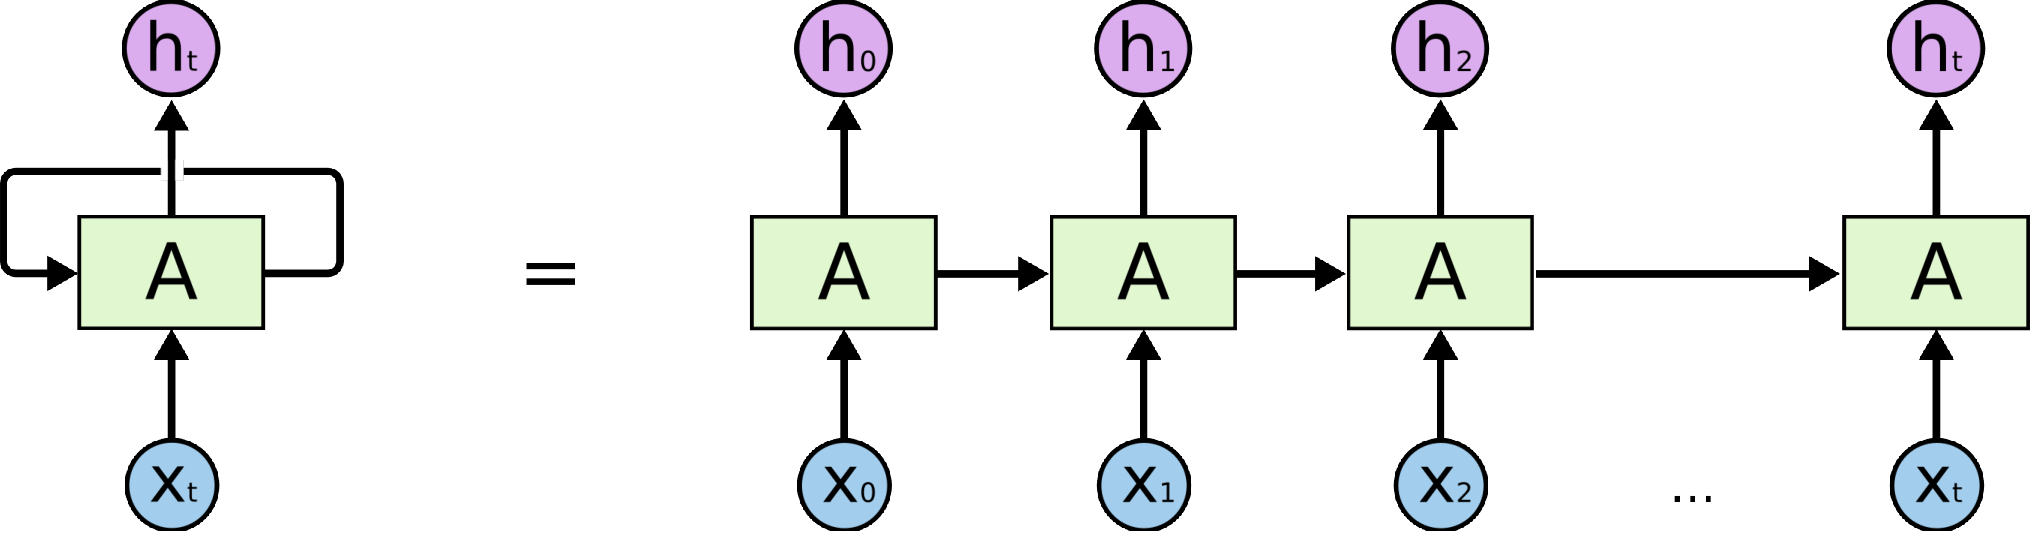
\includegraphics[width=0.5\columnwidth]{RNNUnrolled.pdf} }
\textbf{\caption{A Recurrent Neural Network \cite{olah2015understanding}}
\label{fig:rnn1}}
\end{figure}
For instance basically in a context of sequences of numbers we give as input to the Recurrent Neural Network some of the past numbers. It tries to predict the next number. It does it by trying to learn the behavior of the sequences based on the input given and results it found before.

\subsubsection{Recurrent Neural Network - Long Short-term Memory}
\begin{figure}[t!]
\centering
\begin{minipage}{0.48\textwidth}
\centering
\raisebox{-\height}{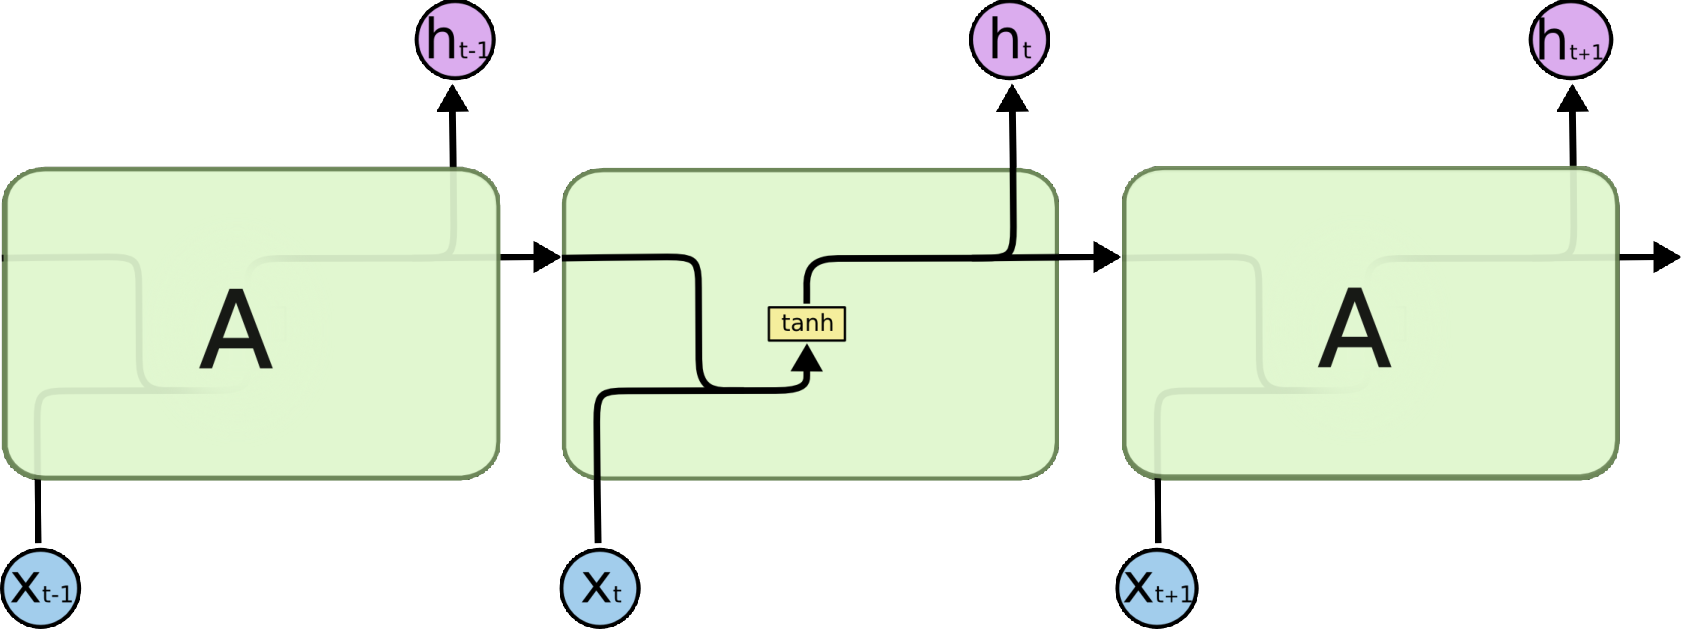
\includegraphics[width=0.8\textwidth]{LSTMSimpleRNN.pdf}}
\textbf{\caption{Simple RNN \cite{olah2015understanding}}
\label{fig:rnn2}}
\end{minipage}
\hfill
\begin{minipage}{0.48\textwidth}
\centering
\raisebox{-\height}{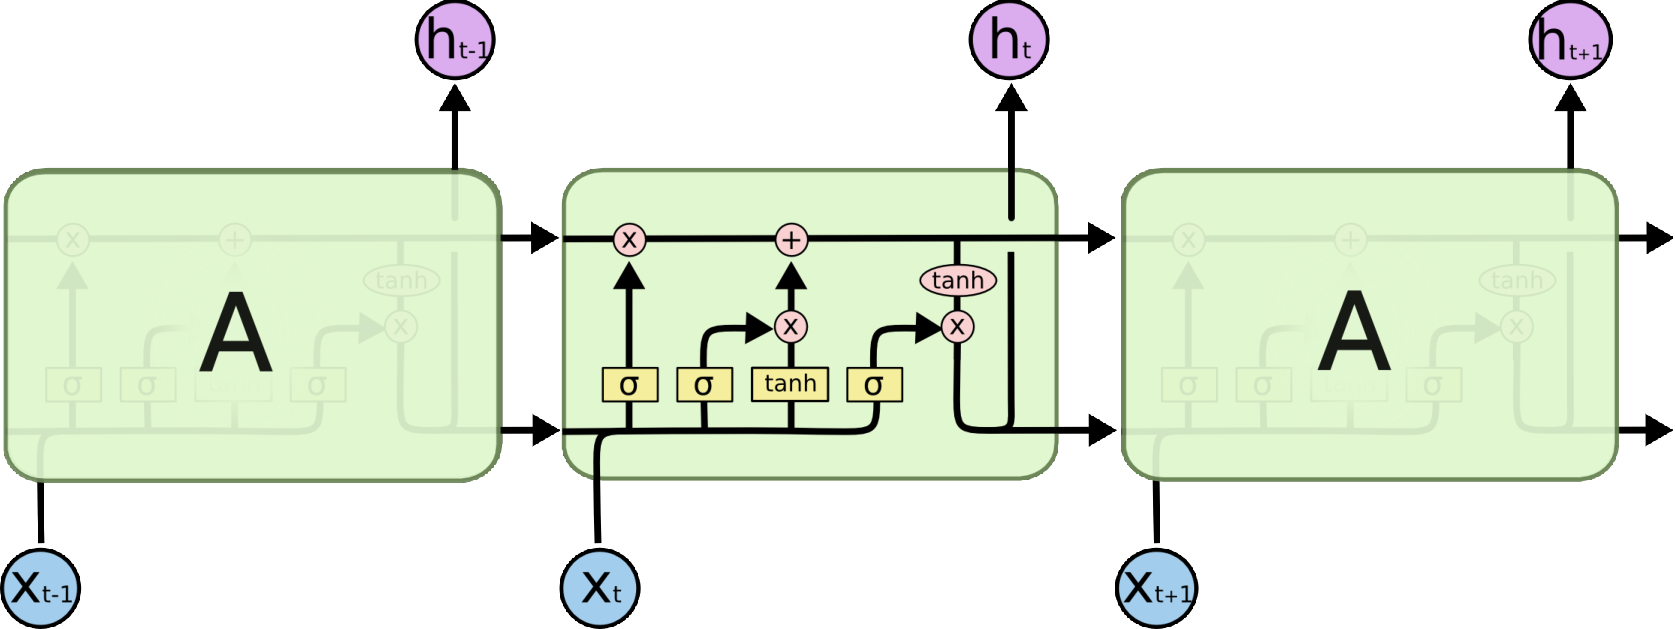
\includegraphics[width=0.8\textwidth]{LSTMchain.pdf}}
\textbf{\caption{RNN-LSTM \cite{olah2015understanding}}
\label{fig:lstm1}}
\end{minipage}
\end{figure}
The Recurrent Neural Network - Long Short-Term Memory (RNN-LSTM) is a special kind of RNN, which is capable of learning really the long-term dependencies. The RNN-LSTM does have the ability to remove, select and add pertinent information from past events. It can really retain important data from previous inputs and use that information to modify its current output. In contrary to a simple RNN which has less control over what kind of data from past events need to be retained an RNN-LSTM introduces a few more control steps. These control steps can be viewed as gates \textit{(See figures: \ref{fig:rnn2} and \ref{fig:lstm1})}. These gates really control the access to the cell state and select which part of the data or previous data will be kept. A RNN-LSTM has a good selective memory even on long-term. It is also why the model is the main model of RNN used in practice. \textit{(See \cite{olah2015understanding} for more details about the model)}


\subsection{Tensorflow}%1/2,1
\begin{figure}[t!]
\centering
\begin{minipage}{0.48\textwidth}
\centering
\raisebox{-\height}{
\includegraphics[width=1\textwidth]{tf.pdf}}
\textbf{\caption{Tensorflow website \cite{tensorflow}}
\label{fig:tf1}}
\end{minipage}
\hfill
\begin{minipage}{0.5\textwidth}
\centering
\raisebox{-\height}{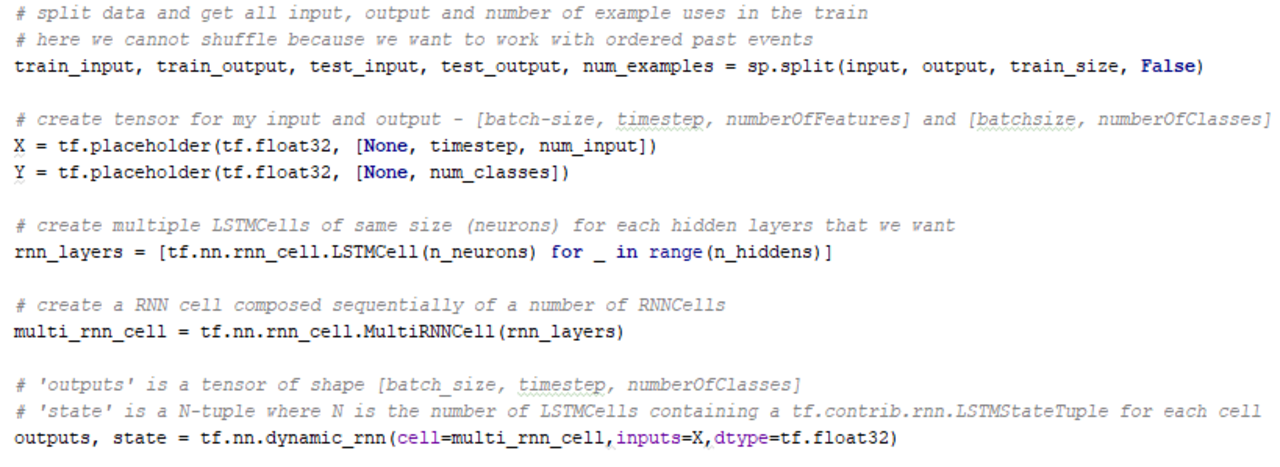
\includegraphics[width=1\textwidth]{tf2b.pdf}}
\textbf{\caption{Some python code with Tensorflow on a multi-layers RNN-LSTM}
\label{fig:tf2}}
\end{minipage}
\end{figure}
Building and using some models for machine learning from the scratch is totally possible. Indeed we only need some mathematics knowledge about it and some skills in programming to do it, but a lot of libraries exist already to optimize it as Torch or MXNet \cite{varangaonkar}. We did not really need to lose time by creating these models from nothing. Tensorflow \cite{tensorflow} is one of these numerous libraries for machine learning and the one we used for our project \textit{(See figures: \ref{fig:tf1} and \ref{fig:tf2})}. This library was developed by Google. First, it was used for internal use in Google, but then it has been released under an open source license. Now it is a free and open source software library. Tensorflow allows us to work with numerical computation using data flow graphs. Without going into details Tensorflow allows working with a large number of models of machine learning or mathematics functions. Moreover, it is portable, the graph (so what we want to do) can be executed immediately or also saved to be used later or reuse. Further, it is flexible and can be run on multiple platforms: CPUs, GPUs, mobile and others. It can also be used with a different level of details. For example, on one side we can use the Keras part of Tensorflow like using machine learning with really fewer needs and knowledge about how works really machine learning, so less control but rapidly useable with pretty good results. On the other side, we can also set and configure all the steps of a model and clearly go into more details about a model. So Tensorflow is really optimal for different purposes whether they are complex or rapid and simple, or even whether the type of users with broad knowledge of machine learning or not.

\subsection{Cesium}%1/2
\begin{figure}[t!]
\centering
\begin{minipage}{0.48\textwidth}
\centering
\raisebox{-\height}{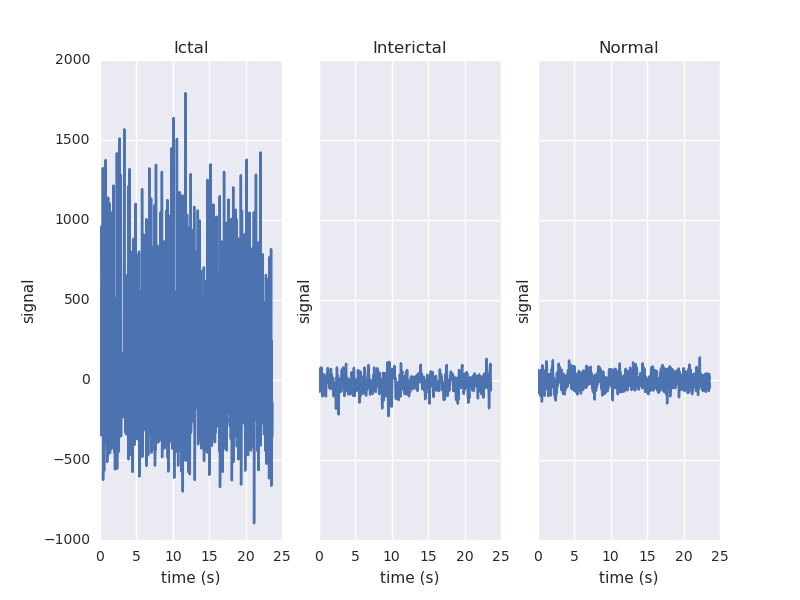
\includegraphics[width=0.7\textwidth]{ces.png}}
\textbf{\caption{Plots \cite{cesium} from EEG time series dataset \cite{andrzejak2001indications}}
\label{fig:ces1}}
\end{minipage}
\hfill
\begin{minipage}{0.5\textwidth}
\centering
\raisebox{-\height}{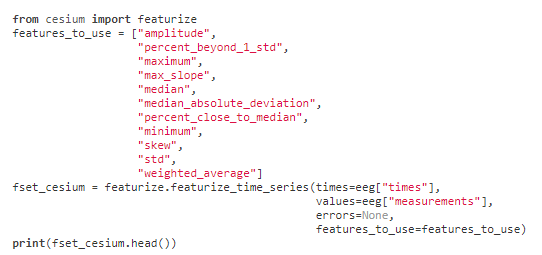
\includegraphics[width=1\textwidth]{ces3a.png}}
\textbf{\caption{Python code with Cesium to extract some selected features from a time series \cite{cesium}}
\label{fig:ces2}}
\end{minipage}
\end{figure}
Cesium \cite{cesium} is also a useful library, but in contrary to Tensorflow it does not work to properly run Machine Learning models. Indeed Cesium is useful in another specific field: time series. Indeed it can extract some really useful information about these kinds of data. It is optimal to extract different features about time series as mean, average, standard deviation but also clearly more complex one as skewness or amplitude of the dataset and a lot many other ones \textit{(See figures: \ref{fig:ces1} and \ref{fig:ces2})}. Furthermore, Cesium can also be used to prepare a model of machine learning based on some of these features or even generate predictions for new data. Concerning its use Cesium works with Python which is a programming language. Moreover, this library is also an open source library. So basically we just need to import the library into Python script. Then through its methods for our case simply select some useful features to extract from the relevant data. So Cesium can be really helpful for some little analysis of time series.

\subsection{Dataset}
\begin{figure}[t!]
\centering
{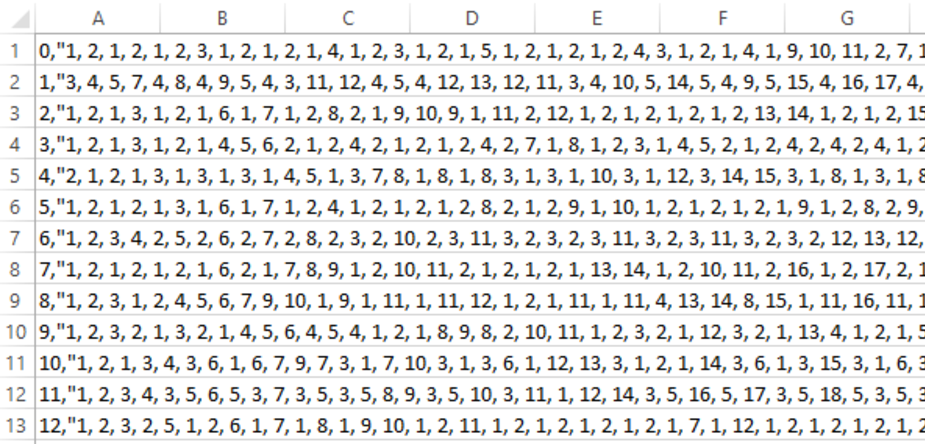
\includegraphics[width=0.75\columnwidth]{db.pdf} }
\textbf{\caption{Dataset where each row represents the movements of one user between POIs}
\label{fig:db}}
\end{figure}
For the project, we have access to a dataset from Nokia. This dataset is interesting in priority because it has the position in the time of some users in their everyday life. A lot of other information was collected in this dataset and are also accessible for us, as for instance message sends, calls, battery level and so one. Moreover, this dataset is interesting especially to us with data about positions of our country and near our region. This dataset contains 150 users that received smartphones to use and keep all time from 2009 to 2011. Smartphones have collected all data possible, as SMS, phone call, network and many more data. It was always done preserving the confidentiality of the users. 

The data that concerns us in priority was geolocation positions of the users in time, basically the longitude, latitude and time per user. With this data, we can begin to use them and work on our subject. After having looked at the datasets, we needed to select a way to begin. Starting directly with positions (longitude, latitude) and time with machine learning is not necessarily the best way; it can be really complex and has bad results. Especially, for the first work on machine learning. We have first simplified the data, by taking only what we call points of interest. These are only some areas on a map where users stay more than a certain time. The data on which we work now is simply movements between these points of interest (POIs). All this data are put in a sequence. We have then a sequence of indexes, where each index represents one of these zones where users stay more than a certain time. For instance, the following sequence [0 1 0 2 3 .... ] will represent the movement of one user. First, he is in the area 0 then goes to 1. Next, he returns to 0, then goes to 2, and so one \textit{(See figure: \ref{fig:db})}. Therefore these sequences have no notion of time, but still respecting the chronological order. In the further work, we can imagine maybe to reuse the first data (longitude, latitude, and time, and also maybe more feature if we think that can help our case) and try to perform better and have also better results.


%----------------------------------------------------------------------------------------
% Related Work
%----------------------------------------------------------------------------------------
\newpage
\section{Related Work}
In the context of machine learning, cases and studies are very wide and numerous. Other people have already worked on a similar or at least a project with some concept in common with ours. Trying to discover and work all by ourselves without according regards to the works of others would be wasting time. Indeed looking at models and researches of others made us win a lot of time to understand similar problems and how to handle them. 
Moreover, people have also worked on the generation of mobility trajectories, but not necessarily about human trajectories. For instance, Technitis Georgios and Weibel Robert \cite{technitis} have worked on a generation of trajectories. They created an algorithm to generate random trajectories between two points for bird migrations. Their models work fine, their trajectories seem good, but still are mainly based on random. Such models based on random give some interesting results but when used with constraints and boundaries. 
For instance, some of the Random walk models give particularly good results for generalized patterns. Indeed the Levy walk model can be used in the case of ocean predators when they can't find food \cite{humphries2010environmental}. These predators abandon their previous pattern to follow a Levy walk model with a mix of long trajectories and short ones. 
Another work related to random which is interesting was the work of Bin Jiang and al \cite{jiang2009characterizing}. They worked also on the subject of generation of mobility trajectories, but in their case about human trajectories. Their purpose was to show that the network of city influences clearly the behavior. They generated the mobility of a large number of random walkers which are forced to follow street network. Then they compared the results with real walkers. It results that random walkers and real one have common behavior. It seems that random can be applied in some specific cases of mobility field.

Another category of models, not necessarily involving random, is mobility models based on some historical traces. For instance, Ghosh et al. \cite{ghosh2017modeling} have worked on finding a way to model human movement behavior, but without connection to random walk model. Indeed they did it by analyzing GPS traces in order to find some correlation between users, places or even a mix of both. Their model is able to categorize the different users based on their traces. It gives us also summaries of the trajectories per category of users. In a similar approach, the work of Kim et al. \cite{kim2006extracting} is interesting. They have also worked on extracting a mobility model based on GPS traces. They found a mobility model where the speed and pause time of the user's movements follow a log-normal distribution, so they find some relationship between some users. The two above studies prove that we can find some common characteristics on users traces, but neither of them resolves the challenge of modeling human mobility for specific behaviors.

In all the above models and techniques, their trajectories can in someways stop suddenly or even turn very sharply. They can fail in really capturing the true movement behaviors of specific people, animal or even objects and can clearly have a mismatch with some particular type of behavior. Jean-Daniel et al. try to avoid a part of this problem of sudden change of trajectories proposed by the common model. They use an Enhanced Gauss-Markov (EGM) mobility model \cite{biomo2014enhanced}. Indeed they try to limit some sudden stops and same cycles within specific regions. Their model ensures nearly only smooth trajectories. Among all these works we see that it is possible to cluster some behaviors based on their similitudes and even to obtain some smooth trajectories. Some facts occur with most of these models; they are based on stochastic process and have not clearly captured human realistic mobility characteristics. Moreover, they don't use some relation to past locations as we want to do. All this consolidates the thought that finding a global model that can work on common behaviors and uncommon ones is quite challenging and yet not found. Furthermore, it pushes us, even more, to try to go further, to really try to capture the behavior of people and generate trajectories. We tried to do it without a goal-oriented to prove some facts about society or human behavior as some of these works have done, and mostly without setting restrictive limits on locations.

%----------------------------------------------------------------------------------------
% Methodology
%----------------------------------------------------------------------------------------
\newpage
\section{Methodology}
Every project needs to have a plan to follow or to try to follow. To achieve the project of generating synthetic mobility trajectories, we divided it into three big phases: Prediction, Optimization, and Generation.

\subsection{Prediction}
The first and important part of the project is to find a model that predicts the trajectories of users based on their previous position(s). For this, we need to check and find a model that performs well and better than a classic model as logistic, linear model or random model. We need to try, execute and compare different models. See how they perform on the dataset available, check where and maybe why one model performs better than others. We need also to try to find their limits. When we are confident in a model and its performances, the next step can begin.

\subsection{Optimization}
After having selected a model on which work, the next step is now to begin to fine-tune it; begin to switch and compare parameters. We need to find an adequate learning rate, a number of epochs during the training (number of time that our train data will pass in our model), number of neurons or the number of hidden layers for a neural network, and so one. We need also to try to go to the limit of the model with the dataset available. A big part of testing, switching some little things, comparing them, and trying to reach conclusions and some results to finally find the best parameters for a model on our data.

\subsection{Generation}
The last part of the project is about generating data based on the model of predictions selected previously. For example by giving a program a starting position and letting the model give the next positions based on how it has predicted it. It is a phase of generating and evaluating the data generated in order to see if it approaches the behavior observed in our datasets. Finally, this phase gives some conclusions about the different methods find for generating synthetic mobility trajectories.


%----------------------------------------------------------------------------------------
% Prediction
%----------------------------------------------------------------------------------------
\newpage
\section{Prediction}
This first part of the project was to create different models of machine learning in order to predict the next positions of users based on their last position or some of their last positions. Then we compared these different models to finally be able to argue in favor of one of them for the next steps of the project. For all that we first began with some data pre-processing to be able to be used in a good way with all our future models.

\subsection{Data Pre-processing}
As described in the section \textit{Dataset}, we have worked on a simplification of the problem with sequences of points of interest (that we called POIs). The first thing was to extract all transitions from users in shape of sequences of POIs. Which mean all data having the form as [0 1 0 2 3 .... ]. Then according to some readings, we choose to represent all positions by a vector binary which represents all POIs possible to have a better shape to work on machine learning. We selected a vector of a shape (1,238) because we identify 238 different areas where users stay more than a certain time. So a position can be represented by this vector of 238 binaries where only one of them will be equal to 1 and will be the index of the position listed. 

\subsection{Prediction Performance}
The models were set up to try to predict the next positions of a user based on their last position or some of their past positions. All models were set with the same simple parameters. We set the learning rate, the batch size, the number of epochs, the training size, the input, the output, the number of timesteps, the number of hidden layers, and the number of neurons. In our case the parameters are defined and first set as following:
\begin{description}
\item [Learning rate] = 0.0001: It can be represented as the speed that the model tries to correct its prediction between training cycles. On one hand, higher the learning rate is, faster the model will change and adapt its prediction, but it will also maybe really put the model in error by going too fast. On the other hand, smaller is the learning rate, slower the model will converge near its best value, but the model will be less likely to miss its apprenticeship and be in error.
\item [Batch size] = 20: It corresponds to the number of input data given to the machine at the same time during training the sessions. If we set it to 20 and we have 100 input data of training, we will have 5 small cycles of training (one for each batch) in order to complete one entire cycle of training (named epoch).
\item [Number of epochs] = 1000: One epoch represents a complete cycle of training. So when the machine has done one epoch, it has received one time all training data on which it has learned. Indeed the number of epochs corresponds to the number of time all training data will pass through the training.
\item [Training size] = 0.7: It is the percentage $p$ of all data that will be used for training. So $1-p$ will be the percentage of data that will be used for testing.
\item [Input]: It is a vector of 238 binaries which represents all the index of POIs of users. For one current position, only one of these binaries is equal to 1, which corresponds to the index of the position.
\item [Output]: It is also a vector but instead of 238 binaries, it is 238 probabilities. So it corresponds to the probabilities of each of this 238 POIs to be the next position. It does not give directly the next position, but we take then the maximum probability obtained from these different POIs and say that the model predicts this one as next position.
\item [Timesteps] 1 until 5: It corresponds to the number of previous positions that will be taken into account to predict the next position. It represents the history of the user movements that will be used to predict his next position. For instance, a timestep set to 2 corresponds to our model to predict the next positions based on the two last positions.
\item [Hidden layers] = 1: It is the number of hidden layers, so it can represent the depth of the brain, its size or it is complexity.
\item [Neurons] = 20: It is the number of neurons per hidden layers. Where each neuron tries to compute a score based on the weights of their relations between them and other cells. So more neurons mean more things trying to be captured by the model on the training data (but does not mean that it will capture useful things).
\end{description}

\subsubsection{Linear Regression}
\begin{figure}[t!]
\centering
\begin{minipage}{0.48\textwidth}
\centering
\raisebox{-\height}{\includegraphics[width=1\textwidth]{Model/Linear/user24Timestep1Hidden1Neurons20Movement.pdf}}
\textbf{\caption{Linear Regression model: True movement vs Prediction with 1 timestep and parameters from table \ref{table:predBasic}}
\label{fig:predLinear1}}
\end{minipage}
\hfill
\begin{minipage}{0.48\textwidth}
\centering
\raisebox{-\height}{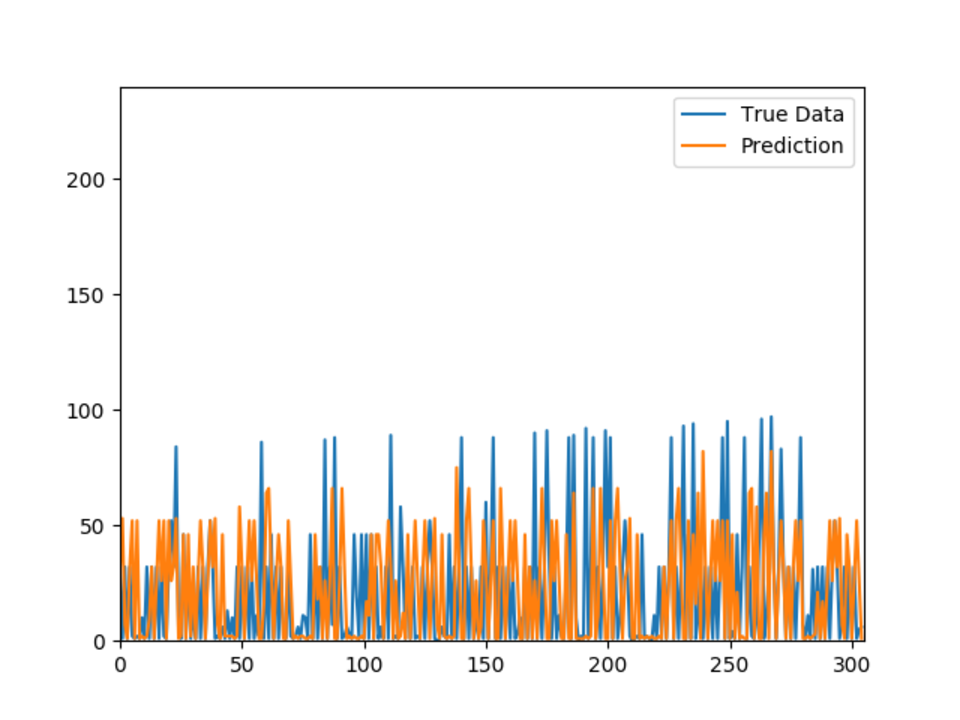
\includegraphics[width=1\textwidth]{Model/Linear/user24Timestep5Hidden1Neurons20Movement.pdf}}
\textbf{\caption{Linear Regression model: True movement vs Prediction with 5 timestep and from table \ref{table:predBasic}}
\label{fig:predLinear2}}
\end{minipage}
\end{figure}

\begin{table}[t!]
\centering
\begin{tabular}{|c|c|c|c|c|}
\hline
\textbf{User}            & \textbf{Learning rate}      & \textbf{Batch size}     & \textbf{Epoch}            & \textbf{Training size}   \\ \hline
\multicolumn{1}{|r|}{24} & \multicolumn{1}{r|}{0.0001} & \multicolumn{1}{r|}{20} & \multicolumn{1}{r|}{1000} & \multicolumn{1}{r|}{0.7} \\ \hline
\end{tabular}
\textbf{\caption{Settings of simple models during prediction}
\label{table:predBasic}}
\end{table}

The Linear model was really a basic model. We did not expect it to work really well. The first result confirmed our thoughts. It was with only one timestep, so by trying to predict the next position with only the last position of the user. It seems that the movement predicted was clearly not good. It did not really fit with the true trajectories linked \textit{(See figure: \ref{fig:predLinear1})}.
Then we tried with more timesteps until 5. It seemed quickly to improve the performance of the predicted positions, even if we used a linear model \textit{(See figure: \ref{fig:predLinear2})}.
These first graphs and results seemed finally not so bad, but to perform better and improve this model, it would be very hard. Indeed this model is a very simple one, without much parameters to change or adapt. This model shows us that even now we can see that some timesteps can really improve results, but it can't really improve the capturing of a human movements behavior. The need for a model that can capture more information and perform better is required.

\subsubsection{Logistic Regression}
The Logistic model was also quite a basic model. Like the linear model we did not expect much of it and the results with only one timestep also proved it to us \textit{(See figure: \ref{fig:predLogistic1})}.
\begin{figure}[t!]
\centering
\begin{minipage}{0.48\textwidth}
\centering
\raisebox{-\height}{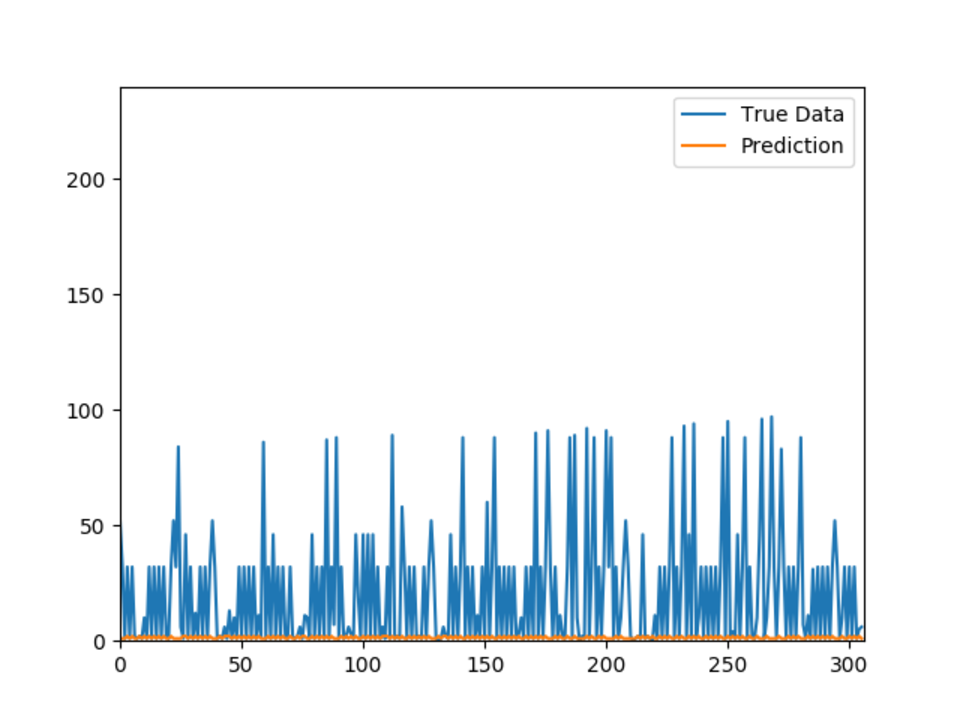
\includegraphics[width=1\textwidth]{Model/Logistic/user24Timestep1Hidden1Neurons20Movement.pdf}}
\textbf{\caption{Logistic Regression model: True movement vs Prediction with 1 timestep and parameters from table \ref{table:predBasic}}
\label{fig:predLogistic1}}
\end{minipage}
\hfill
\begin{minipage}{0.48\textwidth}
\centering
\raisebox{-\height}{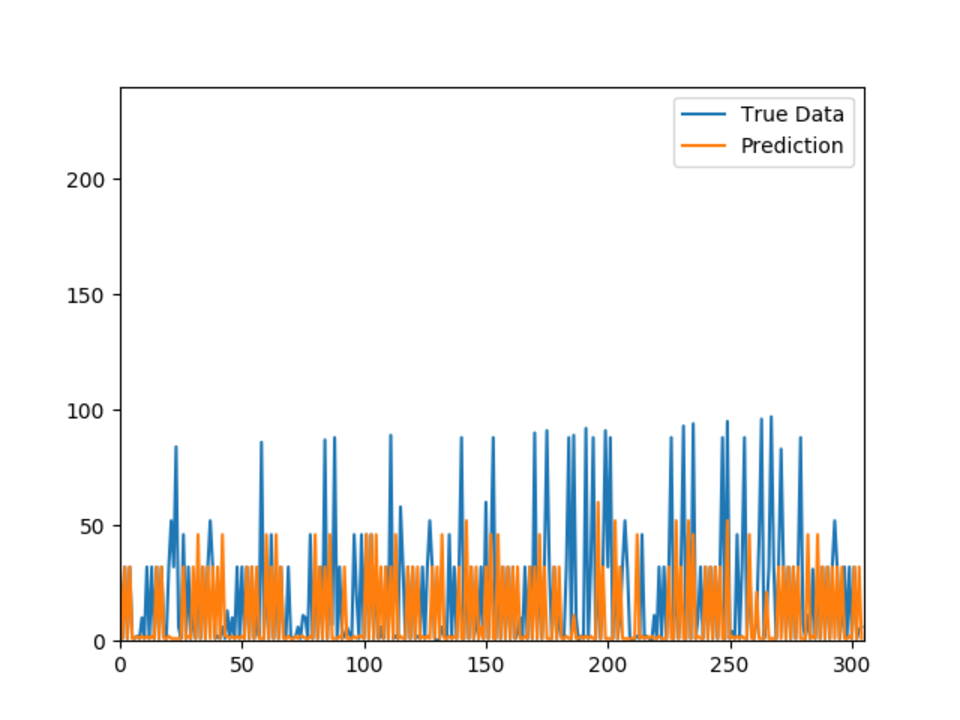
\includegraphics[width=1\textwidth]{Model/Logistic/user24Timestep5Hidden1Neurons20Movement.pdf}}
\textbf{\caption{Logistic Regression model: True movement vs Prediction with 5 timestep and parameters from table \ref{table:predBasic}}
\label{fig:predLogistic2}}
\end{minipage}
\end{figure}
The same effect occurs as with the linear model. Indeed the model shows us that having more timesteps is already better \textit{(See figure: \ref{fig:predLogistic2})}, but really work with it will be hard. Its results seem too much mechanical and without the human touch and as with the Linear Regression model it will be hard to really improve it, because of its lake of parameters and flexibility. It confirms us the need of a model more complex, flexible and that we can really optimize.

\subsubsection{Neural Network}
\begin{table}[t!]
\centering
\begin{tabular}{|c|c|c|c|c|c|c|}
\hline
\textbf{User}            & \textbf{Learning rate}      & \textbf{Batch size}     & \textbf{Epoch}            & \textbf{Training size}   & \textbf{Hidden layer}  & \textbf{Neuron}         \\ \hline
\multicolumn{1}{|r|}{24} & \multicolumn{1}{r|}{0.0001} & \multicolumn{1}{r|}{20} & \multicolumn{1}{r|}{1000} & \multicolumn{1}{r|}{0.7} & \multicolumn{1}{r|}{1} & \multicolumn{1}{r|}{20} \\ \hline
\end{tabular}
\textbf{\caption{Settings of complex models during prediction}
\label{table:predComplex}}
\end{table}

\begin{figure}[t!]
\centering
\begin{minipage}{0.48\textwidth}
\centering
\raisebox{-\height}{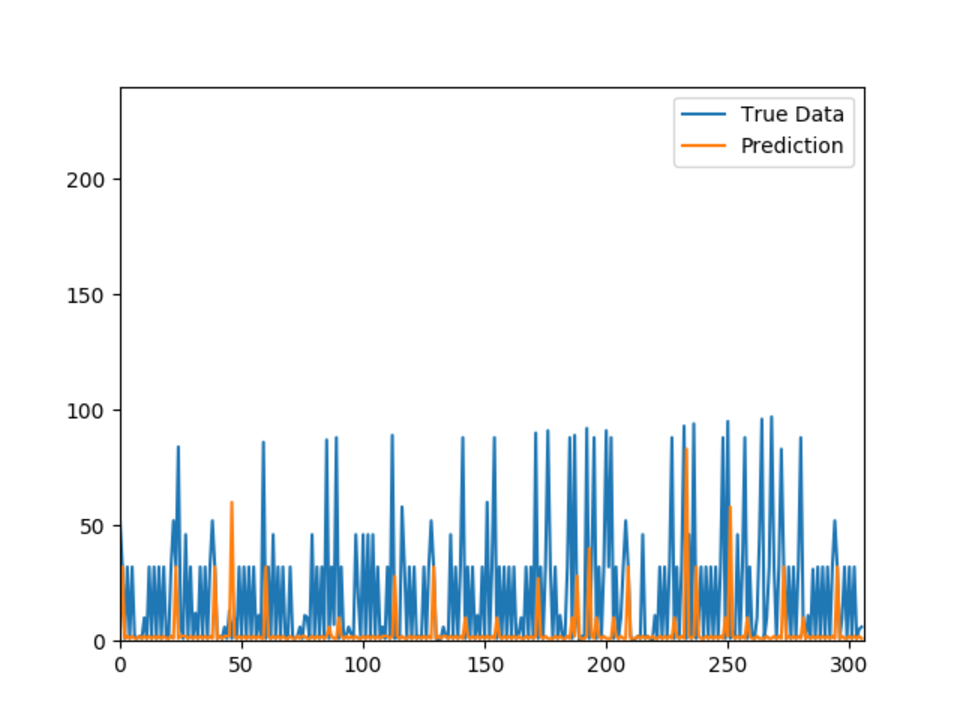
\includegraphics[width=1\textwidth]{Model/NN/user24Timestep1Hidden1Neurons20Movement.pdf}}
\textbf{\caption{Neural Network model: True movement vs Prediction with 1 timestep and parameters from table \ref{table:predComplex}}
\label{fig:predNN1}}
\end{minipage}
\hfill
\begin{minipage}{0.48\textwidth}
\centering
\raisebox{-\height}{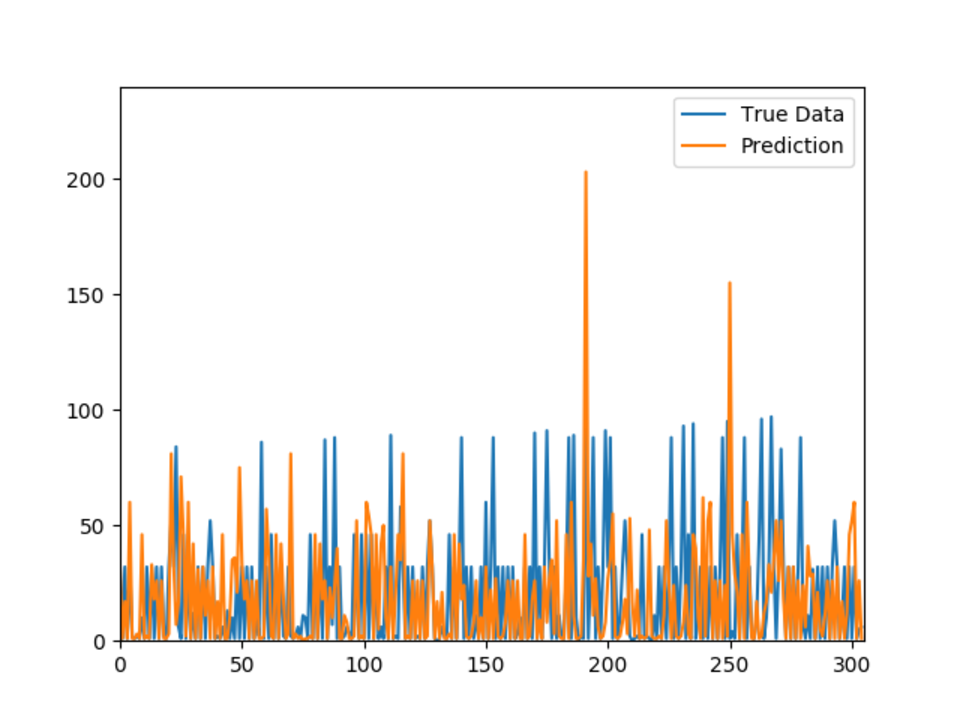
\includegraphics[width=1\textwidth]{Model/NN/user24Timestep5Hidden1Neurons20Movement.pdf}}
\textbf{\caption{Neural Network model: True movement vs Prediction with 5 timestep and parameters from table \ref{table:predComplex}}
\label{fig:predNN2}}
\end{minipage}
\end{figure}
First, the neural network was also disappointing and upset us with its first results with only one timestep \textit{(See figure: \ref{fig:predNN1})}.
It seems also not to be really accurate as the basic models (linear and logistic) for prediction. Then after a second look to really check with more timesteps \textit{(See figure: \ref{fig:predNN2})}, we see that one more time the predictions seems really more near a human behavior.
We can see that even with some basic settings the model is already trying to catch behavior of movement.

\subsubsection{Recurrent Neural Netwok - Long Short-term Memory}
For the RNN-LSTM model, nearly the same effect occurs when we look at trajectory predicted by the model \textit{(See figures: \ref{fig:predLSTM1} and \ref{fig:predLSTM2})}. 
\begin{figure}[t!]
\centering
\begin{minipage}{0.48\textwidth}
\centering
\raisebox{-\height}{\includegraphics[width=1\textwidth]{Model/LSTM/user24Timestep1Hidden1Neurons20Movement.pdf}}
\textbf{\caption{RNN-LSTM model: True movement vs Prediction with 1 timestep and parameters from table \ref{table:predComplex}}
\label{fig:predLSTM1}}
\end{minipage}
\hfill
\begin{minipage}{0.48\textwidth}
\centering
\raisebox{-\height}{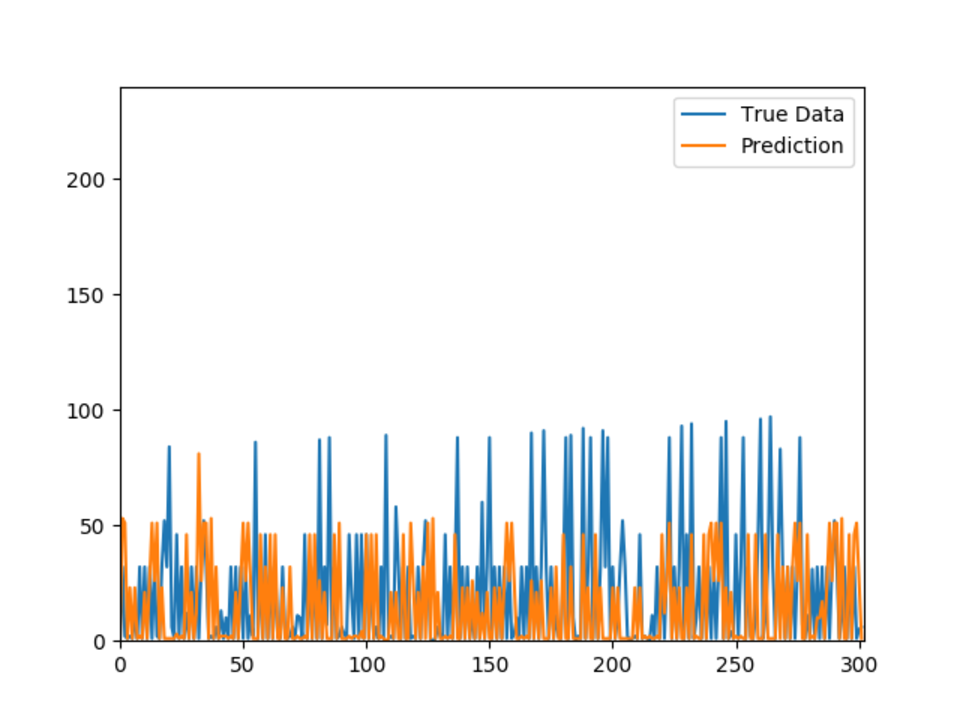
\includegraphics[width=1\textwidth]{Model/LSTM/user24Timestep5Hidden1Neurons20Movement.pdf}}
\textbf{\caption{RNN-LSTM model: True movement vs Prediction with 5 timestep and parameters from table \ref{table:predComplex}}
\label{fig:predLSTM2}}
\end{minipage}
\end{figure}
After having seen the real behavior and compared it with one of the basic models, we can only comfort our first thought; so a more complex model will help us to have better results. Indeed we will be able to improve the model because it has now only very low parameters (1 hidden layers and 20 neurons only). Even more in the next phases; we consolidated even more the fact that having some memory of past information help us to have better results, even if we saw it already a little bit.

\subsection{Overview and Comparison}
In all models used, it seems that they capture some information and behavior from the data given to them, but only the Neural Network and the Recurrent Neural Network seem to give us something near the reality more often than basic models. It will be possible to perform better by trying to change some of the parameters for all these models before selecting one, but already with some basic parameters, we can see that results lean in favor of a more complex model. Moreover as said on the basic models they have fewer parameters to really improve results. Indeed with parameters of the Logistic Regression model and Linear Regression model we can only try to change some basic stuff for their training as the number of epochs, the learning rates, so without really improving or really changing them; it will be as trying to improve a model that is already near its full capacity, so very complicated. In contrary to the NN and RNN-LSTM which can really be modified by changing their complexity by changing their number of neurons or even their number of hidden layers, so basically their size and power. It is why we choose not to spend more time with a basic model and try next to optimize the Recurrent Neural Network: our RNN-LSTM. 

The Neural Network model seemed also really promising, but it is just because we tried to simulate the potential of the RNN-LSTM as with the basic models. Especially we tried to simulate timesteps for having some memory of past events. Trying to continue with the NN was just to simulate the work of the LSTM. It was not really useful, and even more, the way the model received data to simulate some timesteps was only time-consuming during training sessions. Indeed the NN and the two basic models are not able to keep a memory of past information or results. To simulate this memory we simply increased their input data given, so finally, they had really larger inputs when working with more timesteps. For instance, when the RNN-LSTM has always an input size of 238 binaries, the other models had an input of 238 binaries multiplied by the number of timesteps, where each slice of 238 binaries represents one of the last positions. With this practice, it simulates timesteps of the RNN-LSTM and by the way, also has inputs clearly larger. The time that these models take to process it increase drastically with timesteps. It is also why we choose to clearly continue with only the RNN-LSTM.

%----------------------------------------------------------------------------------------
% Optimize
%----------------------------------------------------------------------------------------
\newpage
\section{Optimization}
The next big phase was to try to find the best or at least good parameters for our models, parameters that could give interesting results. The process was to set and test some parameters then try to change them. For this, we tried to select some different range of values for our parameters and tried to compare their results. For instance, we choose to set some parameters as 5 hidden layers, save the results, and then try to increase this number of layers. If the new result was better than the last one, in the next step we continued to increase it, but on the contrary, if the results were worse, we decreased the parameters. Then the same process was done for some of the other parameters. 

It was clear that this task could take a lot of time if knowing that there are 150 data's users to train, so as many models to train. Having time and computer power limited, we choose to only train and make results for a part of our data. We choose to take only 25 users with more data, so in our case more movements between POIs. We choose this number of users because we assumed that users with more data, with more transitions between POIs, would be better than those with few transitions. The fact was that some users had really few data, so few transitions between POIs. Using a big model of machine learning on them as LSTM would have been absurd knowing that this type of machine learning needs normally a lot of data to be correctly trained. The second fact was that users with more movements would have also normally more transitions between different POIs. It would represent globally better our users and their areas visited.

We used our models with different parameters on these users. Thereafter we obtained also different results for each of our 25 users selected. We needed to find a way to say if the model performed good or bad or at least find out if with these parameters it performed better than with other parameters. For that, we select two simple processes to evaluate the results for each set of parameters. Although they are not really purely scientific and are also based on our own opinion, they were an easier and fastest way to choose between parameters: 
\begin{enumerate}
\item Manually by simply looking at the movements predicted for each user and comparing them with some real one.
\item Statistically by selecting some measures that seemed interesting. So these measures were extracted on the movement predicted and the real one, then compared with each other. To selected finally the parameter that seemed to have measures on average nearest to those from true data.
\end{enumerate}

\subsection{Hyperparameter Tuning}
Concerning our parameters in comparison with the ones in the section \textit{Prediction}, we just increased the batch size and the number of epochs. Indeed now we wanted to train the machine with only users that had more transition, so more data. Moreover, we used more complex model with higher parameters, so it would need more training cycles to capture the behavior. Furthermore having more training cycles (epochs) would drastically increase the time spent on training, so we choose to increase the batch size that would speed up the process without having really negative effects on the results. It would maybe even be better with a higher batch size. According to some forum and discussion read; higher the batch is, better is the accuracy of the estimate of the gradient. Having only a batch size of 20 as before was clearly only to process on users with really few transition. Now that we restricted our job to only users with more transitions, the batch size could be higher easily. We set first some basic parameters \textit{(See table \ref{table:optSettings})}.
\begin{table}[t!]
\centering
\begin{tabular}{|c|c|c|c|}
\hline
\textbf{Learning rate} & \textbf{Batch size} & \textbf{Epoch} & \textbf{Training size} \\ \hline
\multicolumn{1}{|r|}{0.0001} & \multicolumn{1}{r|}{100} & \multicolumn{1}{r|}{5000} & \multicolumn{1}{r|}{0.7} \\ \hline
\end{tabular}
\textbf{\caption{Basic settings during optimization}
\label{table:optSettings}}
\end{table}
Then as said some measures were taken into consideration to compare the results of our different settings. These measures were extracted from the predicted trajectories of our models. These trajectories consist of each point predicted by the model based on the last real position or some of the last real positions depending on the number of timesteps. Moreover, most of these measures were extracted from the library \textit{Cesium} as spoken in the section \textit{Background}.
\begin{description}
\item [Mean:] Mean of observed values.
\item [Median:] Median of observed values.
\item [Maximum:] Maximum observed value.
\item [Minimum:] Minimum observed value.
\item [Unique:] Total number of unique observed values. \cite{scipy2}
\item [Std:] Standard deviation of observed values.
\item [Skew:] Skewness of a dataset. Approximately 0 for Gaussian data.
\item [Amplitude:] Half the difference between the maximum and minimum magnitude.
\item [Max slope:] Compute the largest rate of change in the observed data.
\item [Correlation:] The Pearson correlation coefficient measures linear relationship between two datasets. \cite{scipy}
\item [P-value:] The p-value indicates the probability of an uncorrelated system between two datasets. \cite{scipy}
\end{description}

\newpage
\subsubsection{Hidden layer(s)}
\begin{figure}[t!]
\centering
\begin{minipage}{0.3\textwidth}
\centering
\raisebox{-\height}{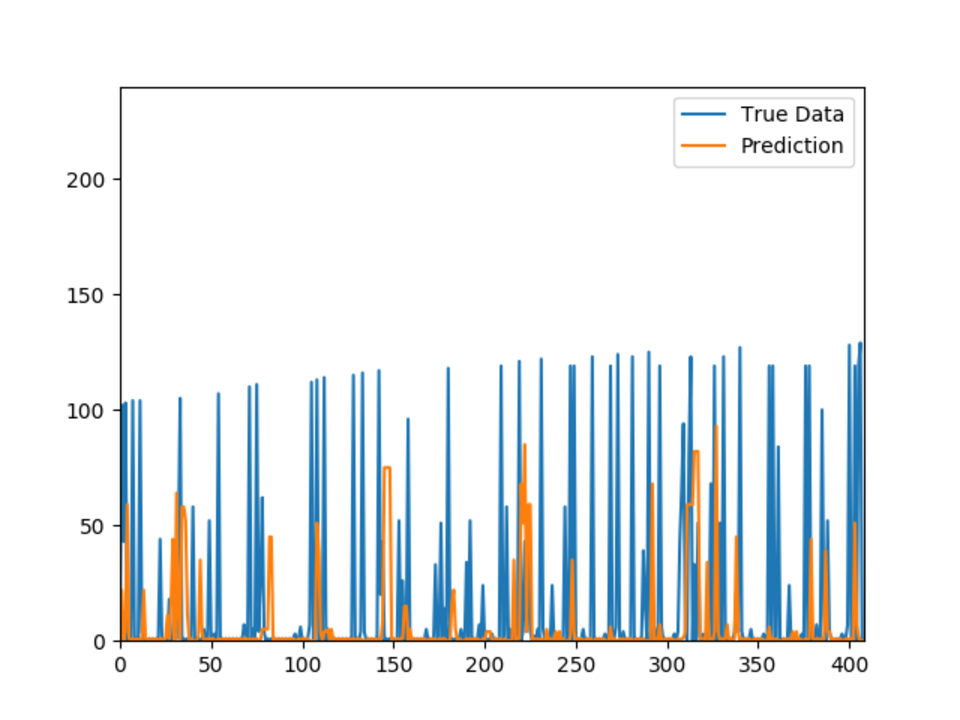
\includegraphics[width=1.1\textwidth]{Optimize/Hidden/user4Timestep5Hidden1Neurons50Movement.pdf}}
\textbf{\caption{True movement vs Prediction (1 hidden layer)}
\label{fig:optH1}}
\end{minipage}
\hfill
\begin{minipage}{0.3\textwidth}
\centering
\raisebox{-\height}{\includegraphics[width=1.1\textwidth]{Optimize/Hidden/user4Timestep5Hidden5Neurons50Movement.pdf}}
\textbf{\caption{True movement vs Prediction (5 hidden layers)}
\label{fig:optH2}}
\end{minipage}
\hfill
\begin{minipage}{0.3\textwidth}
\centering
\raisebox{-\height}{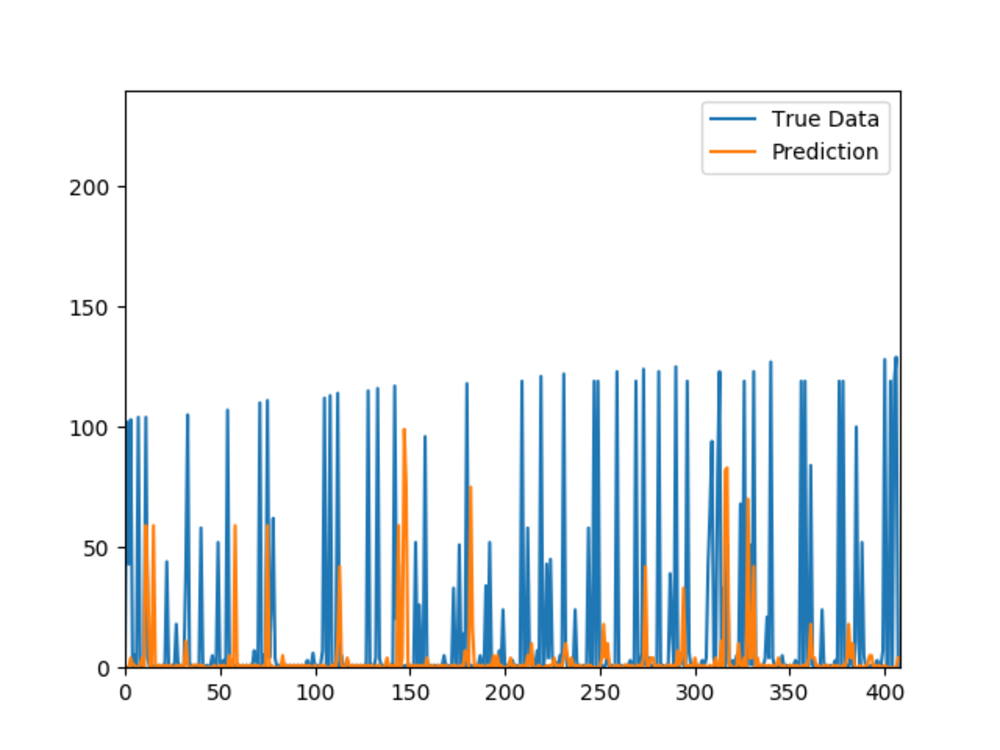
\includegraphics[width=1.1\textwidth]{Optimize/Hidden/user4Timestep5Hidden10Neurons50Movement.pdf}}
\textbf{\caption{True movement vs Prediction (10 hidden layers)}
\label{fig:optH3}}
\end{minipage}
\end{figure}
\begin{table}[t!]
\centering
\begin{tabular}{l|r|r|r|r|r|r|r|}
\cline{2-8}
& \multicolumn{1}{l|}{\textbf{1 HL}} & \multicolumn{1}{l|}{\textbf{3 HL}} & \multicolumn{1}{l|}{\textbf{5 HL}} & \multicolumn{1}{l|}{\textbf{7HL}} & \multicolumn{1}{l|}{\textbf{10 HL}} & \multicolumn{1}{l|}{\textbf{20 HL}} & \multicolumn{1}{l|}{\textbf{Real}} \\ \hline
\multicolumn{1}{|l|}{\textbf{Mean}} & 15.003 & 16.361 & 17.843 & 17.175 & 14.21 & 5.426 & 22.012 \\ \hline
\multicolumn{1}{|l|}{\textbf{Median}} & 5.86 & 8.32 & 8.48 & 7.64 & 8.0 & 2.82 & 9.52 \\ \hline
\multicolumn{1}{|l|}{\textbf{Maximum}} & 106.56 & 108.72 & 110.2 & 106.76 & 104.76 & 76.24 & 133.12 \\ \hline
\multicolumn{1}{|l|}{\textbf{Minimum}} & 0.2 & 0.16 & 0.16 & 0.2 & 0.2 & 0.32 & 0.12 \\ \hline
\multicolumn{1}{|l|}{\textbf{Unique}} & 27.68 & 33.64 & 36.2 & 34.8 & 25.72 & 9.36 & 47.08 \\ \hline
\multicolumn{1}{|l|}{\textbf{Std}} & 22.158 & 23.982 & 25.169 & 24.334 & 21.54 & 10.134 & 33.279 \\ \hline
\multicolumn{1}{|l|}{\textbf{Skew}} & 2.842 & 2.598 & 2.489 & 2.478 & 3.189 & 5.753 & 2.226 \\ \hline
\multicolumn{1}{|l|}{\textbf{Amplitude}} & 53.18 & 54.28 & 55.02 & 53.28 & 52.28 & 37.96 & 66.5 \\ \hline
\multicolumn{1}{|l|}{\textbf{Max slope}} & 104.24 & 106.36 & 107.6 & 104.44 & 102.2 & 74.12 & 130.48 \\ \hline
\multicolumn{1}{|l|}{\textbf{Correlation}} & 0.082 & 0.06 & 0.056 & 0.044 & 0.023 & 0.013 & 1.0 \\ \hline
\multicolumn{1}{|l|}{\textbf{P-value}} & 0.328 & 0.335 & 0.315 & 0.435 & 0.457 & 0.384 & 0.0 \\ \hline
\end{tabular}
\centering
\textbf{\caption{Some measures from different number of hidden layers and true movement}
\label{table:hidden}}
\end{table}
First, the tests were to find the best number of hidden layers, so we tried different numbers: 1,3,5,7,10 and 20.
The result was pretty obvious that 5 hidden layers were clearly better than less or more layers if the model has 50 neurons per hidden layers and timesteps of 5. We can see some features extracted from generating path predicted (point by point) of our different results and the real mean based on true movement from our users in the following table. We see clearly that 5 hidden layers perform nearly always a little bit better than the others. Especially when we look to the \textit{Mean} and \textit{Median} which is with \textit{Correlation} and \textit{P-value} the measures that we look in priority. Only for the \textit{Correlation} and \textit{Skew} the model with 5 hidden layers was not the best, but so nearly from the best results \textit{(See table: \ref{table:hidden})}.
Moreover, for instance, with the following graphs that compare movement generated point by points, it seems that 5 hidden layers are better than a unique hidden layer. It is also clear that the model with 5 hidden layers tries to capture more transitions and clearly more different positions \textit{(See figures: \ref{fig:optH1} and  \ref{fig:optH2})}.
Then we can also see that more hidden layers decrease a lot the results \textit{(See figure: \ref{fig:optH3})}. It seems that the model with too many hidden layers begins to only predict the POIs with more occurrences. We can presume different effects. Maybe there are too few training cycles or even that the model is too complex for this data as we try to calculate a simple addition with a powerful computer while a simple calculator can do the job.
However, all these results seem to be in favor of 5 hidden layers. So we kept these parameters for the following.

\subsubsection{Neurons}
The next tests were to find a good number of neurons per layer. It was set to 50 during the last tests, so then we tried to increase, decrease and compare them: 10,20,50,70,100 and 150 neurons per layers. So we found that the best number of neurons was approximately 50 with 5 hidden layers and 5 timesteps. 
We can see it here that too few neurons per hidden layer will clearly decrease results \textit{(See table: \ref{table:neuron})}. In the same way, too many neurons will not really improve results and will just increase drastically the training time. Based on the measures of this table we can assume that 50 neurons are the best choice. The model with 50 neurons per layers obtains the best results for 5 of these measures; Mean, Median, Minimum, Correlation and P-value. Moreover, this model never has a measure with really bad results comparing to other models. When it performs less well than another model, it is always really near to the best value obtained by the best model. Furthermore looking at the movement predicted compared to a real one, it confirms clearly that taking fewer neurons than 50 is a bad choice \textit{(See figures: \ref{fig:optN1} and \ref{fig:optN2})}.
In the same way, it confirms that too many neurons will not really improve results \textit{(See figure: \ref{fig:optN3})} and as said will just increase the training time.
We set neurons per hidden layers to 50 for the following.
\begin{figure}[t!]
\centering
\begin{minipage}{0.3\textwidth}
\centering
\raisebox{-\height}{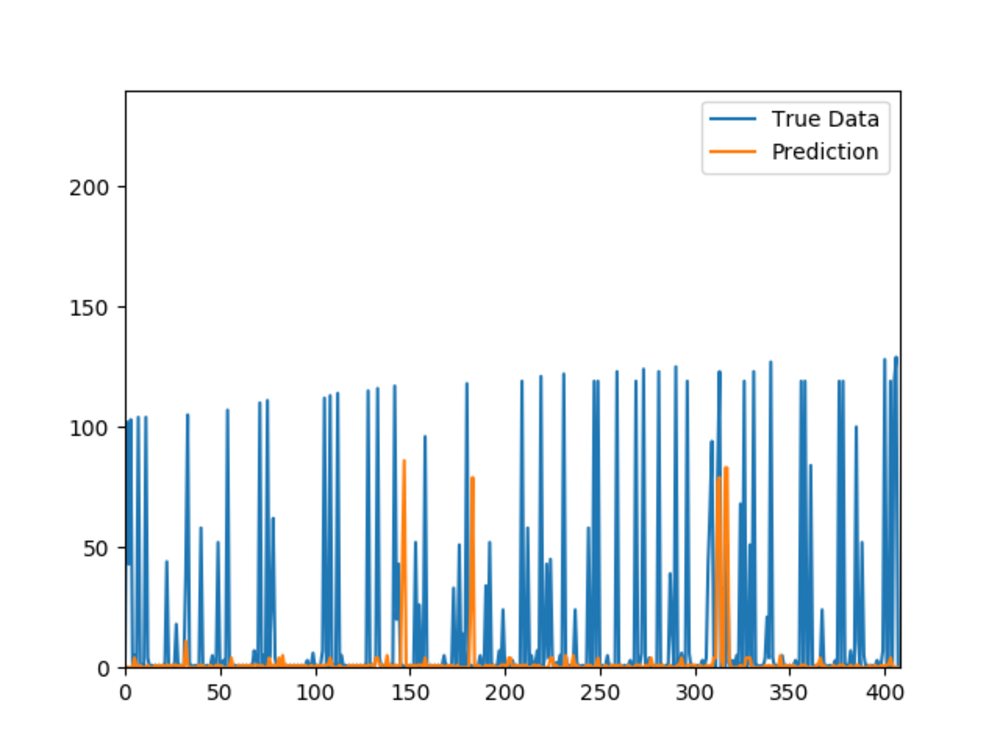
\includegraphics[width=1.1\textwidth]{Optimize/Neuron/user4Timestep5Hidden5Neurons10Movement.pdf}}
\textbf{\caption{True movement vs Prediction with 10 neurons}
\label{fig:optN1}}
\end{minipage}
\hfill
\begin{minipage}{0.3\textwidth}
\centering
\raisebox{-\height}{\includegraphics[width=1.1\textwidth]{Optimize/Neuron/user4Timestep5Hidden5Neurons50Movement.pdf}}
\textbf{\caption{True movement vs Prediction with 50 neurons}
\label{fig:optN2}}
\end{minipage}
\hfill
\begin{minipage}{0.3\textwidth}
\centering
\raisebox{-\height}{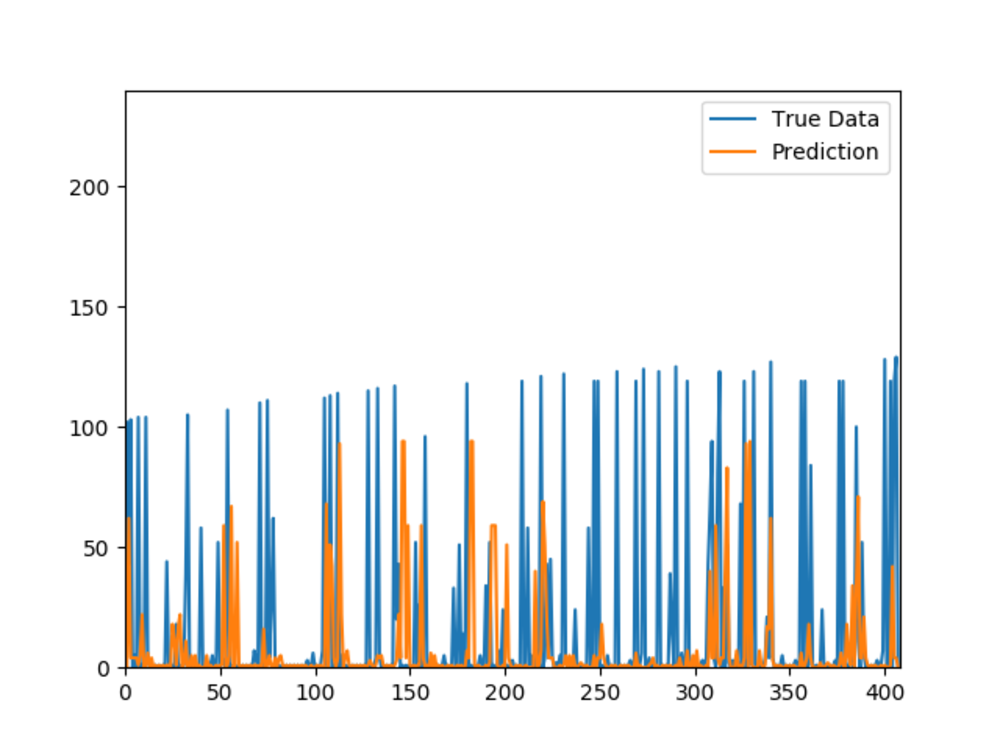
\includegraphics[width=1.1\textwidth]{Optimize/Neuron/user4Timestep5Hidden5Neurons100Movement.pdf}}
\textbf{\caption{True movement vs Prediction with 100 neurons}
\label{fig:optN3}}
\end{minipage}
\end{figure}

\begin{table}[t!]
\centering
\begin{tabular}{l|r|r|r|r|r|r|r|}
\cline{2-8}
& \multicolumn{1}{l|}{\textbf{10 N}} & \multicolumn{1}{l|}{\textbf{20 N}} & \multicolumn{1}{l|}{\textbf{50 N}} & \multicolumn{1}{l|}{\textbf{70 N}} & \multicolumn{1}{l|}{\textbf{100 N}} & \multicolumn{1}{l|}{\textbf{150 N}} & \multicolumn{1}{l|}{\textbf{Real}} \\ \hline
\multicolumn{1}{|l|}{\textbf{Mean}} & 10.151 & 14.435 & 17.843 & 17.417 & 17.655 & 17.398 & 22.012 \\ \hline
\multicolumn{1}{|l|}{\textbf{Median}} & 5.28 & 7.88 & 8.48 & 4.92 & 5.86 & 8.3 & 9.52 \\ \hline
\multicolumn{1}{|l|}{\textbf{Maximum}} & 91.08 & 103.56 & 110.2 & 110.28 & 111.6 & 121.72 & 133.12 \\ \hline
\multicolumn{1}{|l|}{\textbf{Minimum}} & 0.28 & 0.24 & 0.16 & 0.16 & 0.2 & 0.16 & 0.12 \\ \hline
\multicolumn{1}{|l|}{\textbf{Unique}} & 11.08 & 21.44 & 36.2 & 38.28 & 36.0 & 36.6 & 47.08 \\ \hline
\multicolumn{1}{|l|}{\textbf{Std}} & 15.604 & 21.742 & 25.169 & 25.22 & 25.492 & 25.142 & 33.279 \\ \hline
\multicolumn{1}{|l|}{\textbf{Skew}} & 5.071 & 3.198 & 2.489 & 2.378 & 2.456 & 3.175 & 2.226 \\ \hline
\multicolumn{1}{|l|}{\textbf{Amplitude}} & 45.4 & 51.66 & 55.02 & 55.06 & 55.7 & 60.78 & 66.5 \\ \hline
\multicolumn{1}{|l|}{\textbf{Max slope}} & 88.84 & 100.2 & 107.6 & 106.2 & 109.96 & 119.44 & 130.48 \\ \hline
\multicolumn{1}{|l|}{\textbf{Correlation}} & 0.026 & 0.039 & 0.056 & 0.047 & 0.041 & 0.031 & 1.0 \\ \hline
\multicolumn{1}{|l|}{\textbf{P-value}} & 0.448 & 0.454 & 0.315 & 0.46 & 0.45 & 0.417 & 0.0 \\ \hline
\end{tabular}
\centering
\textbf{\caption{Some measures from different number of neurons and true movement}
\label{table:neuron}}
\end{table}

\subsubsection{Timesteps}
Then the last set of tests was to find the best timesteps, so the best memory of last positions to take into account for predictions. Tests were done with different timesteps: 1,3,5,7 and 10 timesteps. It resulted that 5 timesteps are better with our measures. Indeed for this particular user, the model with more timesteps seems good, but when we look at our measures we see clearly the superiority of having 5 timesteps \textit{(See table: \ref{table:timestep})}.
These measures show that increasing the number of timesteps will first rapidly increase nearly all measures until 5 timesteps. After that, if we continue to increase the number of timesteps we can see nearly no more improving. Moreover, it can result by even become worse for some measures as the median compared with the real one. So here it clearly is better to choose the model with 5 timesteps. Indeed this model performs clearly better with the median than any other models. Moreover, all its other measures are always near the best value and never clearly beaten by another model. Furthermore looking at the movement predicted compared to a real one, it confirms clearly that taking fewer timesteps than 5 is a really bad choice \textit{(See figures: \ref{fig:optT1} and \ref{fig:optT2})}.
It is less obvious that too many timesteps are bad with the same type of graph, but we can still conclude that more timesteps don't really improve the results \textit{(See figure: \ref{fig:optT3})}.It is why we set the timesteps to 5 for the following of the project.
\begin{figure}[t!]
\centering
\begin{minipage}{0.3\textwidth}
\centering
\raisebox{-\height}{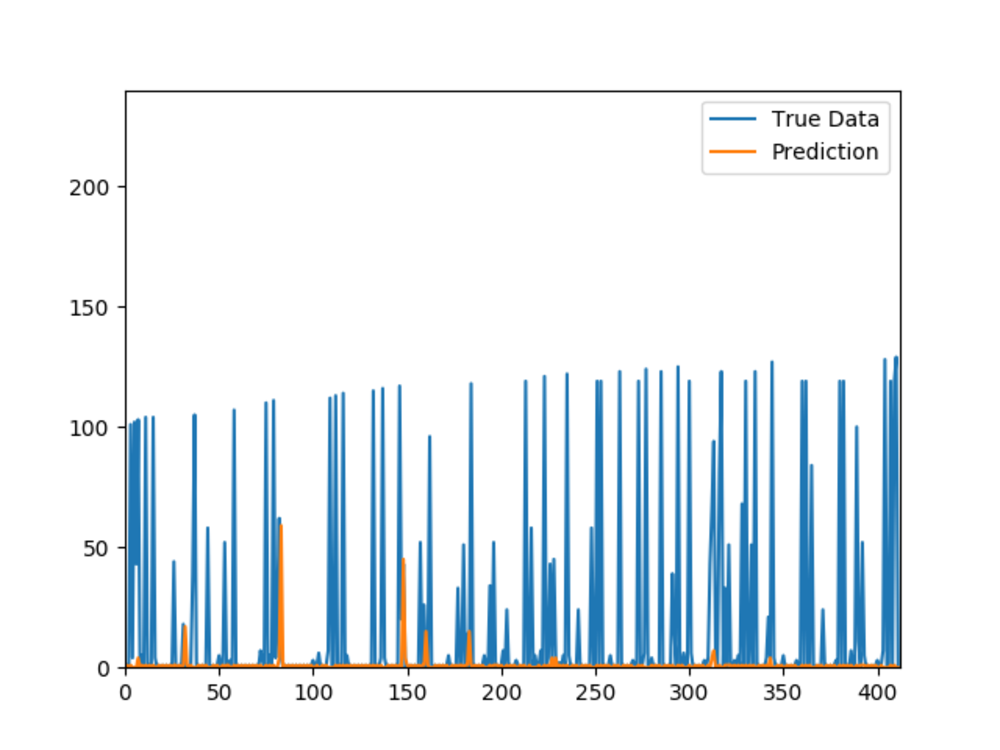
\includegraphics[width=1.1\textwidth]{Optimize/Timesteps/user4Timestep1Hidden5Neurons50Movement.pdf}}
\textbf{\caption{True movement vs Prediction with 1 timestep}
\label{fig:optT1}}
\end{minipage}
\hfill
\begin{minipage}{0.3\textwidth}
\centering
\raisebox{-\height}{\includegraphics[width=1.1\textwidth]{Optimize/Timesteps/user4Timestep5Hidden5Neurons50Movement.pdf}}
\textbf{\caption{True movement vs Prediction with 5 timesteps}
\label{fig:optT2}}
\end{minipage}
\hfill
\begin{minipage}{0.3\textwidth}
\centering
\raisebox{-\height}{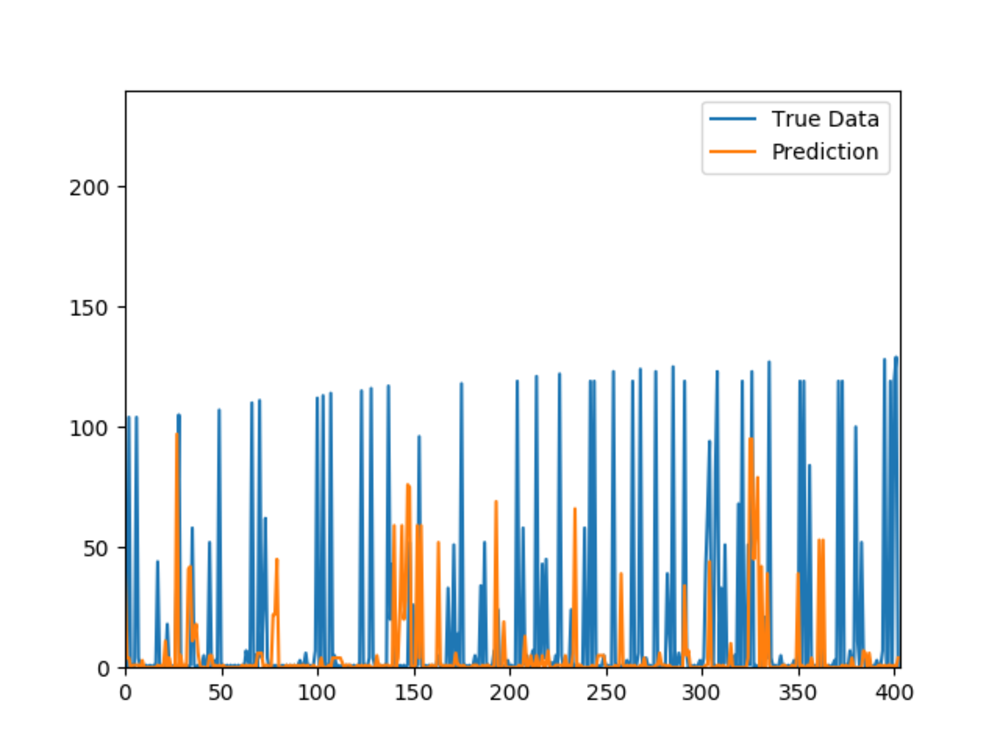
\includegraphics[width=1.1\textwidth]{Optimize/Timesteps/user4Timestep10Hidden5Neurons50Movement.pdf}}
\textbf{\caption{True movement vs Prediction with 10 timestep}
\label{fig:optT3}}
\end{minipage}
\end{figure}

\begin{table}[t!]
\centering
\begin{tabular}{l|r|r|r|r|r|r|}
\cline{2-7}
& \multicolumn{1}{l|}{\textbf{1 T}} & \multicolumn{1}{l|}{\textbf{3 T}} & \multicolumn{1}{l|}{\textbf{5 T}} & \multicolumn{1}{l|}{\textbf{7 T}} & \multicolumn{1}{l|}{\textbf{10 T}} & \multicolumn{1}{l|}{\textbf{Real}} \\ \hline
\multicolumn{1}{|l|}{\textbf{Mean}} & 4.068 & 13.565 & 17.843 & 17.47 & 17.692 & 22.012 \\ \hline
\multicolumn{1}{|l|}{\textbf{Median}} & 1.96 & 3.38 & 8.48 & 5.64 & 5.36 & 9.52 \\ \hline
\multicolumn{1}{|l|}{\textbf{Maximum}} & 62.2 & 107.12 & 110.2 & 108.48 & 110.68 & 133.12 \\ \hline
\multicolumn{1}{|l|}{\textbf{Minimum}} & 0.28 & 0.16 & 0.16 & 0.16 & 0.2 & 0.12 \\ \hline
\multicolumn{1}{|l|}{\textbf{Unique}} & 6.44 & 27.72 & 36.2 & 38.36 & 36.32 & 47.08 \\ \hline
\multicolumn{1}{|l|}{\textbf{Std}} & 7.008 & 22.41 & 25.169 & 25.47 & 25.896 & 33.279 \\ \hline
\multicolumn{1}{|l|}{\textbf{Skew}} & 6.444 & 3.097 & 2.489 & 2.318 & 2.296 & 2.226 \\ \hline
\multicolumn{1}{|l|}{\textbf{Amplitude}} & 30.96 & 53.48 & 55.02 & 54.16 & 55.24 & 66.5 \\ \hline
\multicolumn{1}{|l|}{\textbf{Max slope}} & 60.68 & 105.16 & 107.6 & 106.88 & 108.2 & 130.48 \\ \hline
\multicolumn{1}{|l|}{\textbf{Correlation}} & 0.034 & 0.079 & 0.056 & 0.01 & 0.017 & 1.0 \\ \hline
\multicolumn{1}{|l|}{\textbf{P-value}} & 0.342 & 0.282 & 0.315 & 0.565 & 0.494 & 0.0 \\ \hline
\end{tabular}
\centering
\textbf{\caption{Some measures from different number of timesteps and true movement}
\label{table:timestep}}
\end{table}

\subsection{Overview and Observation}
All tests made and results found show us that it can be complex to find the optimal parameters. Moreover, that trying all combinations of parameters cannot be done without a lot of time spent on training on the machine. We also saw that some parameters obtain better results on some measures than our final selected parameters but on average worse. Indeed machine learning model s like RNN-LSTM can be really complicated and the results are sometimes surprising. It is really hard to know exactly why some parameters work better on some measures than other parameters. Our tests can still conclude some points:
\begin{enumerate}
\item Some hidden layers can capture better long-term dependencies. Indeed 5 hidden layers perform well, especially to approach the real mean and median.
\item Some neurons also perform better than too few. Indeed near 50 neurons, it seems to obtain the best results, especially for the median, mean and P-value.
\item Some timesteps will really try to capture and understand the movement of users. It will know some previous positions to really predict the next position based on the previous path. It clearly increases the results, especially about the median and the mean. Indeed a model with 5 timesteps seems again to perform better on the median and the mean. 
\item Too much-hidden layers, neurons or timesteps will clearly increase a lot the time spent on training without really helping to capture better the behavior of user movements and can even obtain worse results 
\item Not enough hidden layers or neurons will result in having really similar results than a simple model as linear regression or logistic regression. Indeed it will be as having a model which could capture only too few information on the data.
\item To few timesteps will never capture long-term dependencies. It will result in a simple Markov chain during the prediction, so with only the current state (position) that will influence the prediction. It will not, in our case, try to understand the movement of users, but only predict the most likely next position based on occurrences of positions.
\end{enumerate}
We found that the parameters from table \ref{table:optFinal} seem to respond well to prediction. It is why we set them as optimal parameters, in order to keep them for the last phase: Generation. 
\begin{table}[t!]
\centering
\begin{tabular}{|c|c|c|c|c|c|c|}
\hline
\textbf{Learning rate} & \textbf{Batch size} & \textbf{Epoch} & \textbf{Training size} & \textbf{Hidden layer} & \textbf{Neuron} & \textbf{Timestep} \\ \hline
\multicolumn{1}{|r|}{0.0001} & \multicolumn{1}{r|}{100} & \multicolumn{1}{r|}{5000} & \multicolumn{1}{r|}{0.7} & \multicolumn{1}{r|}{5} & \multicolumn{1}{r|}{50} & \multicolumn{1}{r|}{5} \\ \hline
\end{tabular}
\textbf{\caption{Best parameters found}
\label{table:optFinal}}
\end{table}


%----------------------------------------------------------------------------------------
% Trajectory Generating
%----------------------------------------------------------------------------------------
\newpage
\section{Generation}
Now to generate the trajectories, it had no need to run a lot of different models. A global model was trained with all our data. A new model based on the previous best parameters found but trained with all the users. The model can give us a vector of 238 probabilities for the next position based on the last 5 positions (timesteps 5). The sum of all 238 probabilities equals 1. So we have two ways to generate the trajectories based on the model:
\begin{enumerate}
\item By giving the model every time the last 5 positions and select the position predicted that has the highest probability in our output vector of 238 probabilities.
\item By giving the model every time the last 5 positions and select randomly between the 238 positions based on their probabilities in the output (the vector of 238). Therefore a position with a higher probability will have more chance to be generated for the next position than a position with a low probability.
\end{enumerate}
The first method is presumed better when we try to generate few steps. Indeed it will generate the most likely next positions in term of probability, but it is also more susceptible to go in a wrong cycle by predicting always the same movement. The second method can be better to go out of the same cycle of movements because even some POIs that are uncommon will be sometimes (rarely) predicted, so generated. This behavior is more logical to generate large steps. Indeed a user goes sometimes out of his recurrent path. 

\subsection{Random Generator}
In order to confirm our first thought that random model cannot capture a real human behavior, we used as a first generator of trajectories one only based on random. This generator is only to show us that if we only rely on random it does not work and moreover that our other generators give clearly better results. So it just generates the next positions randomly among the point of interests \textit{(See figure: \ref{fig:genR1})}.

\subsection{Best Probability Generator}
The second generator only based on the best probability predicted. It really relies on our global model of prediction with the parameters found in the last section. The global RNN-LSTM model gives us probabilities for the next position. The Best Probability Generator simply always takes the POIs with the highest probabilities for its next positions. Indeed it only needs that we give it five first positions and then it can begin to generate a trajectory for these positions. We can clearly see that the path that it generates seems to have a recurrent behavior or at least some cycles \textit{(See figure: \ref{fig:genN1})}. Moreover, we can notice that this generator will nearly always give the same results for the same input given. It doe does not use rely on a random process.

\subsection{Random Choice Probability Generator}
\begin{figure}[t!]
\centering
\begin{minipage}{0.3\textwidth}
\centering
\raisebox{-\height}{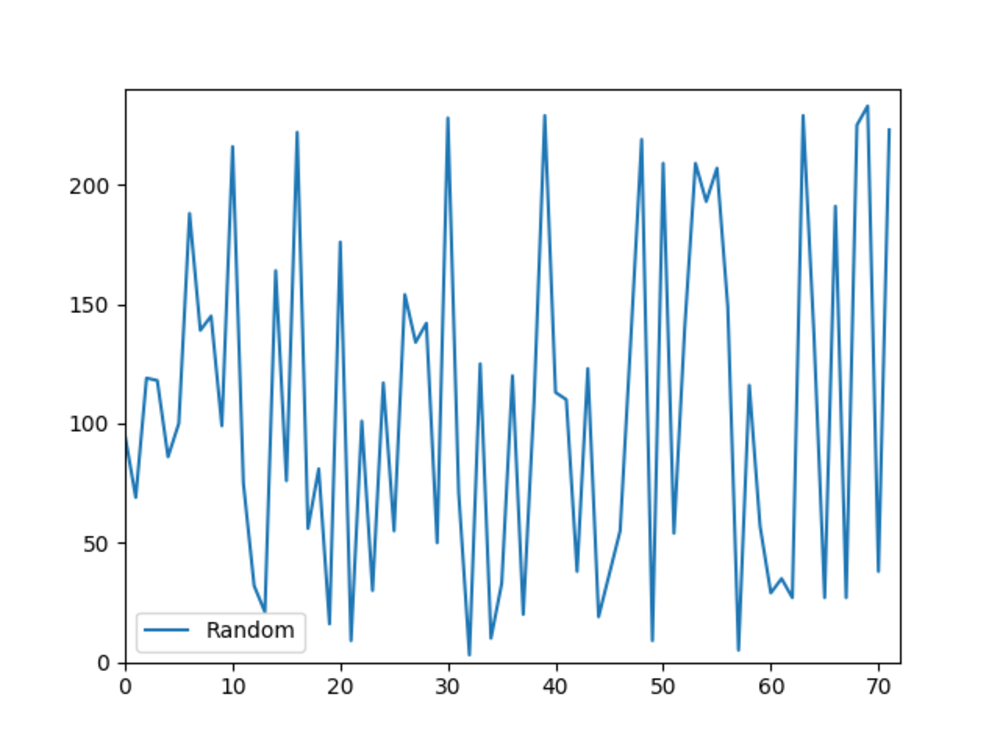
\includegraphics[width=1.1\textwidth]{Generate/Random.pdf}}
\textbf{\caption{Trajectory generated with Random Generator}
\label{fig:genR1}}
\end{minipage}
\hfill
\begin{minipage}{0.3\textwidth}
\centering
\raisebox{-\height}{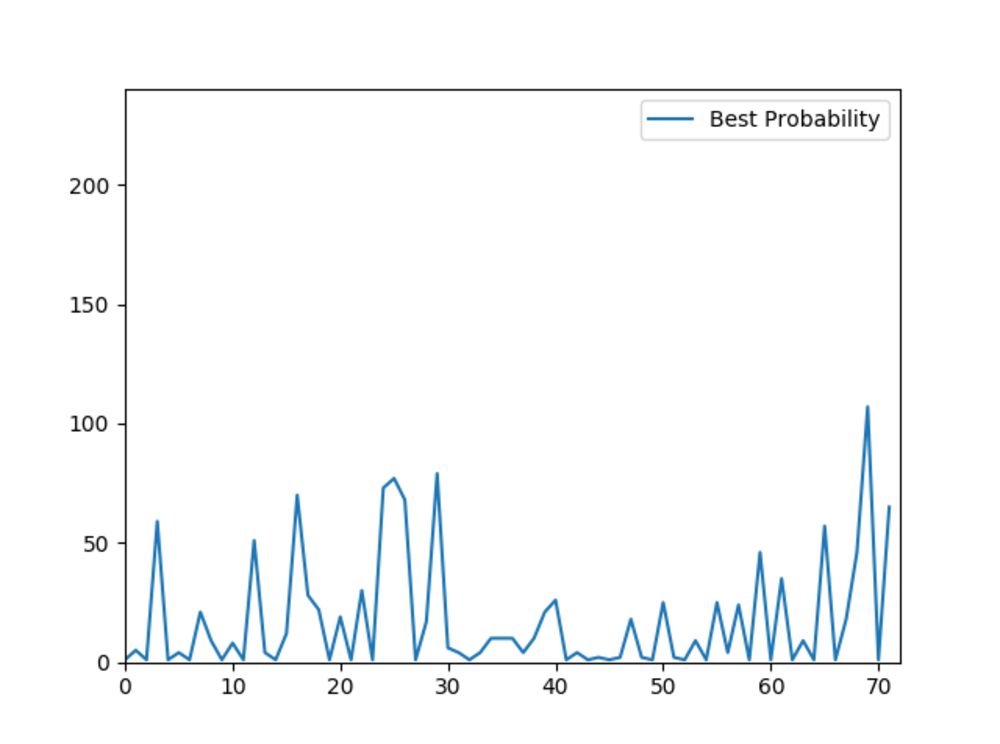
\includegraphics[width=1.1\textwidth]{Generate/Normal.pdf}}
\textbf{\caption{Trajectory generated with Best Probability Generator}
\label{fig:genN1}}
\end{minipage}
\hfill
\begin{minipage}{0.3\textwidth}
\centering
\raisebox{-\height}{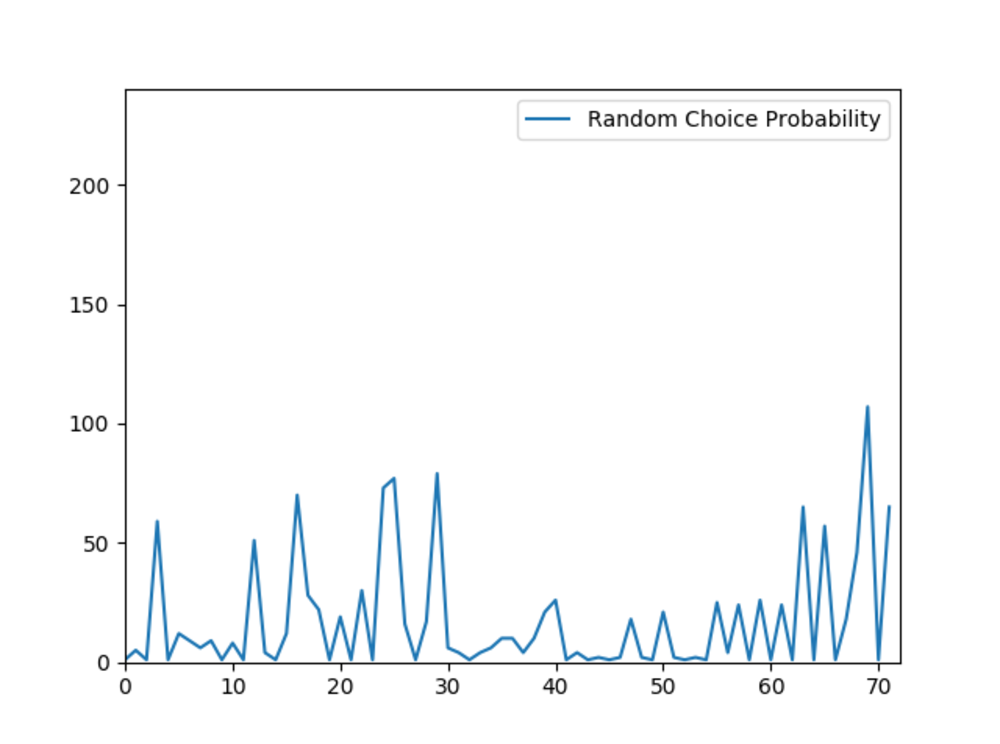
\includegraphics[width=1.1\textwidth]{Generate/Choice.pdf}}
\textbf{\caption{Trajectory generated with Random Choice Probability Generator}
\label{fig:genC1}}
\end{minipage}
\end{figure}
The third generator is also based on probabilities predicted by the global RNN-LSTM model of predictions, but instead of just taking the higher probability it is also based a little bit on random. It combines probability and random choice. It will use the RNN-LSTM model to have the probabilities of all POIs for the next positions and then it will generate next position randomly in taking into account their probabilities. In other words, POIs with a higher probability will more likely be generated. Doing like this the method allows the path generated not to go in a repeated cycle of same movements or same positions. Moreover, it is not totally random because it is based on the probabilities given by the RNN-LSTM model. With this process, we try to simulate the fact that trajectories go sometimes in another way than the most recurrent. 
We can think of a man going every day to work; he will nearly every day go on the same path, but maybe sometimes will choose or be forced to take another path. Maybe because of too much traffic jam, maybe because he needs to look for somebody or even just simply because he is bored by this same path or he wants to try a new path. Even if, as said, this generator uses random, we see also that it is firstly based on the RNN-LSTM predictions; so it uses a bit of random based on behavior captures from users \textit{(See figure: \ref{fig:genC1})}.


\subsection{Performance and Comparison}
\begin{figure}[t!]
\centering
\begin{minipage}{0.3\textwidth}
\centering
\raisebox{-\height}{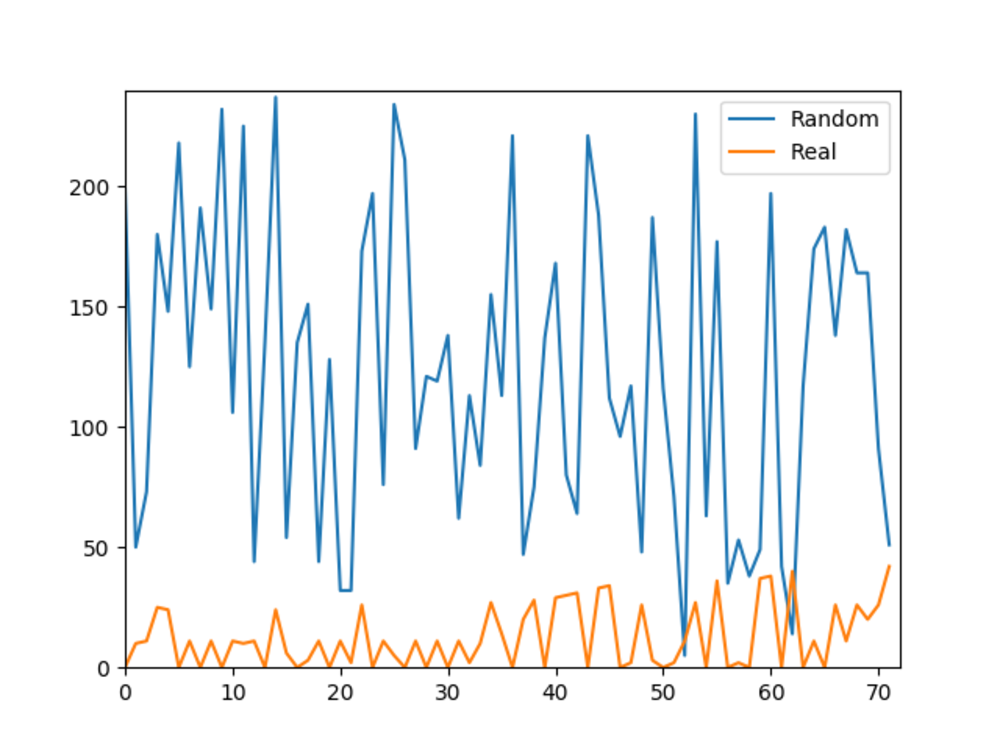
\includegraphics[width=1.1\textwidth]{Generate/H5N50T5/user109Random.pdf}}
\textbf{\caption{Random Generated Trajectory vs Real Trajectory}
\label{fig:genR2}}
\end{minipage}
\hfill
\begin{minipage}{0.3\textwidth}
\centering
\raisebox{-\height}{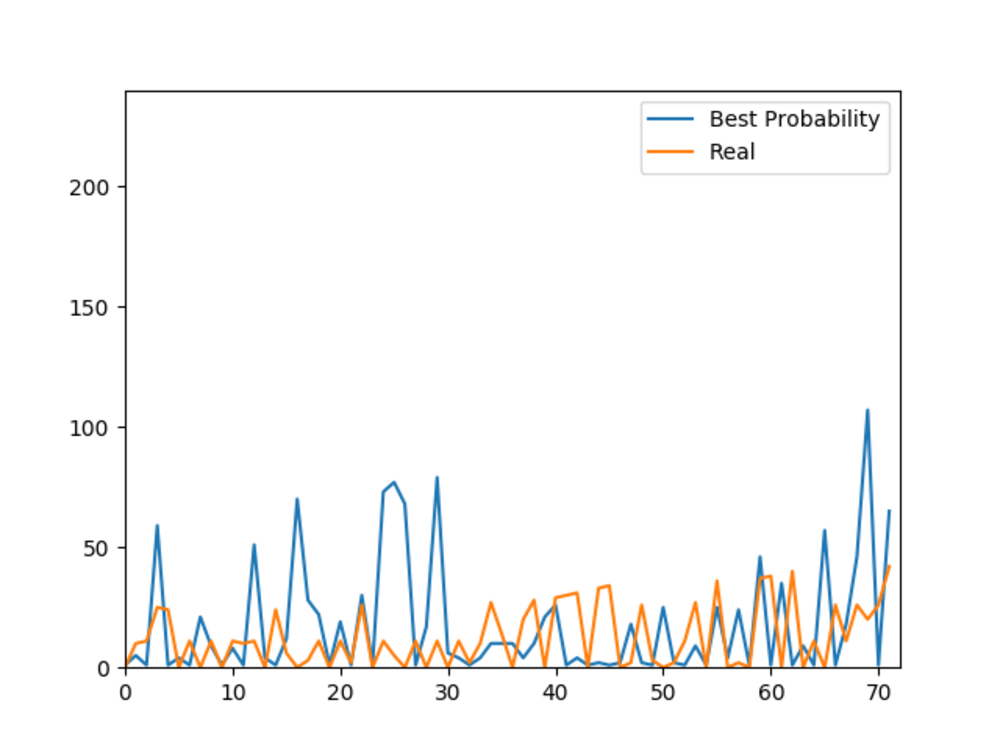
\includegraphics[width=1.1\textwidth]{Generate/H5N50T5/user109Normal.pdf}}
\textbf{\caption{Best Probability Generated Trajectory vs Real Trajectory}
\label{fig:genN2}}
\end{minipage}
\hfill
\begin{minipage}{0.3\textwidth}
\centering
\raisebox{-\height}{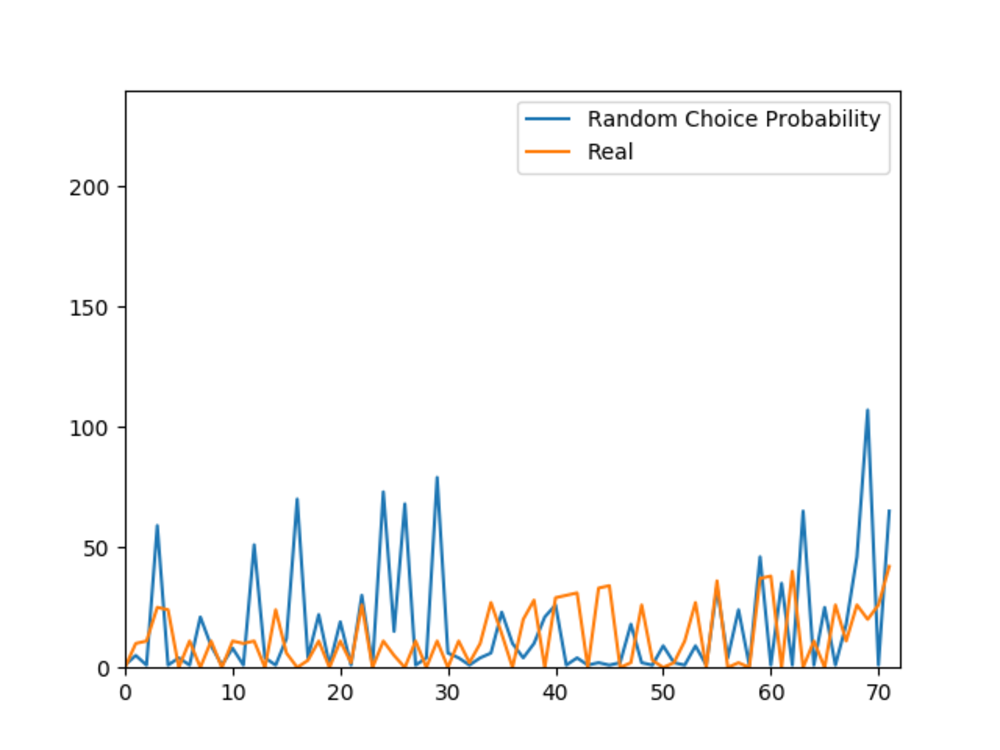
\includegraphics[width=1.1\textwidth]{Generate/H5N50T5/user109Choice.pdf}}
\textbf{\caption{Random Choice Probability Generated Trajectory vs Real Trajectory}
\label{fig:genC2}}
\end{minipage}
\end{figure}
In order to really compare performances, we plot the generated path and a true path to see how they differed. For instance, the Random Generator obtains really bad performances. Indeed we can clearly see that, when we speak about the Random Walk Model, a generator based principally on random cannot capture a real or similar behavior than a human one. It is really obvious that for all spoken applications of trajectories, we can really not take a generator like this one \textit{(See figure: \ref{fig:genR2})}.
For our Best Probability Generator, we also compared a real trajectory with a generated one. We gave this generator simply the first 5 real positions from the true path and then it generated the next positions based on the RNN-LSTM model predictions. We see that this generator is really better than the random one. We can see that it tries to capture a human behavior \textit{(See figure: \ref{fig:genN2})}.
Then for our Random Choice Probability Generator, we also compared a real path with a generated one from it. As for the Best Probability Generator it needs simply the first 5 real positions from a true path and then it generates the next positions based on the LSTM model predictions, but with some random choice. We see that this generator is really better than the random one. We can see that it tries to capture a human behavior \textit{(See figure: \ref{fig:genC2})}. It clearly also seems to be more human than the Random Generator.

\begin{figure}[t!]
\centering
\begin{minipage}{0.48\textwidth}
\centering
\raisebox{-\height}{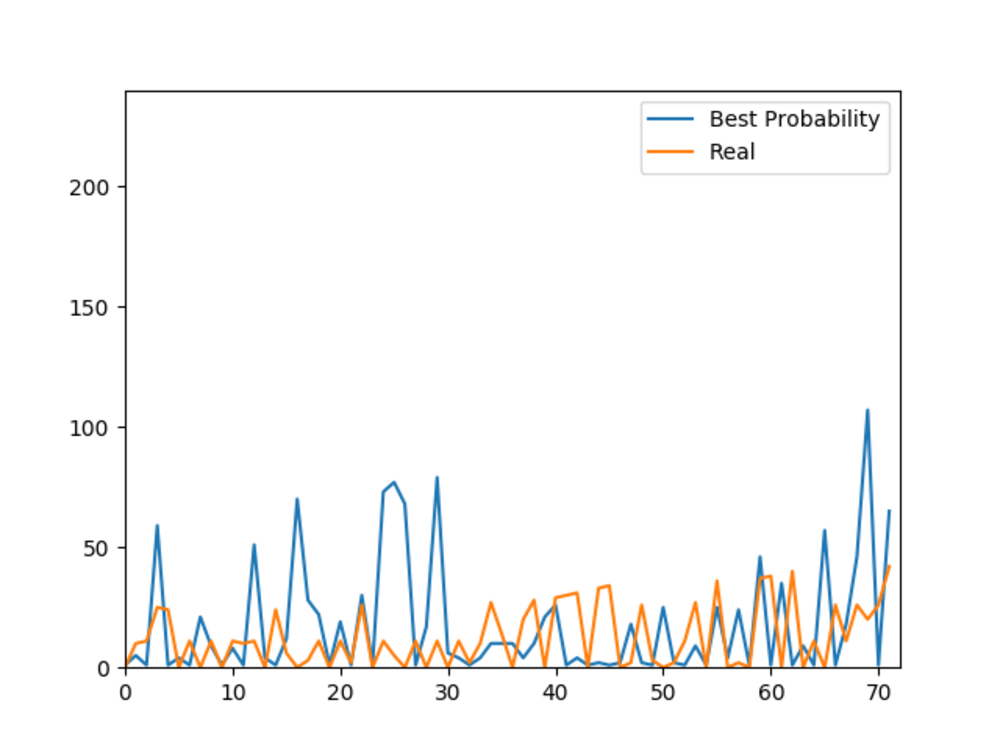
\includegraphics[width=1\textwidth]{Generate/H5N50T5/user109Normal.pdf}}
\textbf{\caption{Best Probability Generator with less than 100 steps}
\label{fig:genN3}}
\end{minipage}
\hfill
\begin{minipage}{0.48\textwidth}
\centering
\raisebox{-\height}{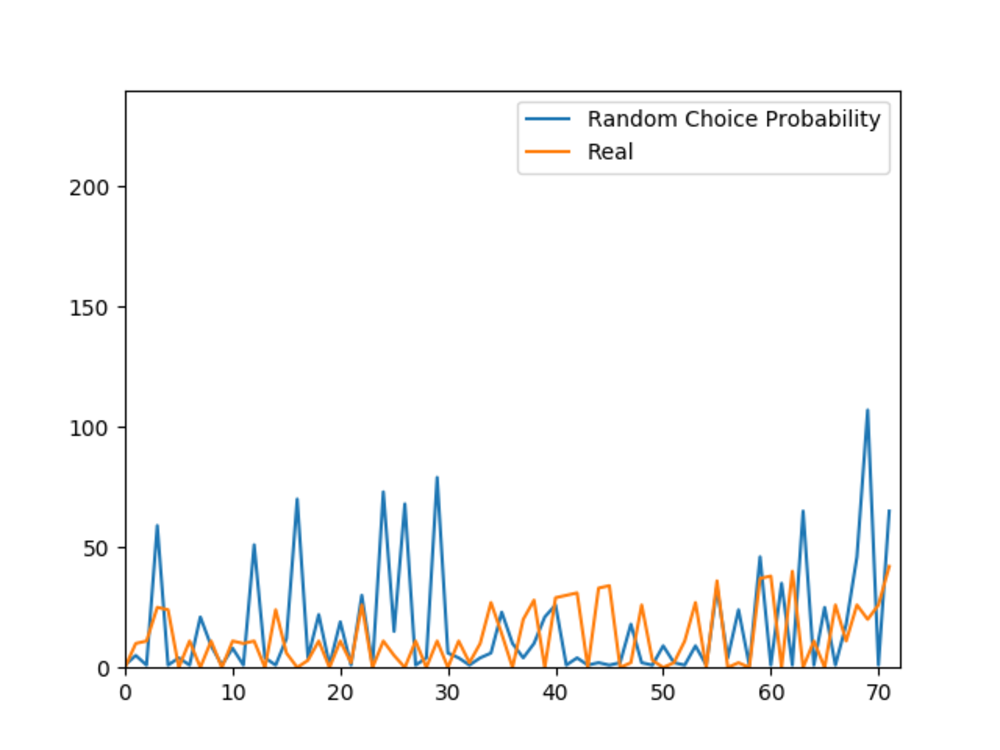
\includegraphics[width=1\textwidth]{Generate/H5N50T5/user109Choice.pdf}}
\textbf{\caption{Random Choice Probability Generator with less than 100 steps}
\label{fig:genC3}}
\end{minipage}
\end{figure}
\begin{table}[t!]
\centering
\begin{tabular}{l|r|r|r|r|}
\cline{2-5}
\textbf{}                         & \multicolumn{1}{c|}{\textbf{Random}} & \multicolumn{1}{c|}{\textbf{Best Probability}} & \multicolumn{1}{c|}{\textbf{Random Choice Probability}} & \multicolumn{1}{c|}{\textbf{Real}} \\ \hline
\multicolumn{1}{|l|}{Mean}        & 118.229                              & 3.78                                           & 8.213                                                   & 17.009                             \\ \hline
\multicolumn{1}{|l|}{Median}      & 117.81                               & 2.2                                            & 2.72                                                    & 8.3                                \\ \hline
\multicolumn{1}{|l|}{Maximum}     & 234.48                               & 50.007                                         & 106.047                                                 & 82.827                             \\ \hline
\multicolumn{1}{|l|}{Minimum}     & 2.013                                & 0.293                                          & 0.073                                                   & 0.413                              \\ \hline
\multicolumn{1}{|l|}{Unique}      & 122.087                              & 9.747                                          & 27.953                                                  & 30.393                             \\ \hline
\multicolumn{1}{|l|}{Std}         & 68.005                               & 7.301                                          & 16.928                                                  & 22.919                             \\ \hline
\multicolumn{1}{|l|}{Skew}        & -0.006                               & 4.571                                          & 3.57                                                    & 1.737                              \\ \hline
\multicolumn{1}{|l|}{Amplitude}   & 116.233                              & 24.857                                         & 52.987                                                  & 41.207                             \\ \hline
\multicolumn{1}{|l|}{Max slope}   & 219.68                               & 47.28                                          & 103.893                                                 & 80.667                             \\ \hline
\multicolumn{1}{|l|}{Correlation} & -0.011                               & 0.009                                          & 0.006                                                   & 1.0                                \\ \hline
\multicolumn{1}{|l|}{P-value}     & 0.498                                & 0.455                                          & 0.498                                                   & 0.0                                \\ \hline
\end{tabular}
\centering
\textbf{\caption{Some measures extracted from the synthetical trajectories of the different generators}
\label{table:generators}}
\end{table}

Based on the above results, we can forget the Random generator, but what about the other two. They really seem to have similar results, even if the measures extracted lean in favor of the last generator \textit{(See table: \ref{table:generators})}. Indeed when we look at each of their generated trajectories, they both capture the human behavior \textit{(See figures: \ref{fig:genN3} and \ref{fig:genC3})}. 
It is why to really see a difference we choose to generate more steps, even though we have not enough true data to compare with. The generated paths obtained at this moment was clearly on average in favor of the Random Choice Probability Generator. Indeed this generator continues to create path have a human behavior. On the contrary, the Best Probability Generator nearly always seems to fall in recurrent cycles of same POIs generated \textit{(See figures: \ref{fig:genN4} and \ref{fig:genC4})}. Moreover, the measures extracted confim it again \textit{(See table: \ref{table:generators2})}.
\begin{figure}[t!]
\centering
\begin{minipage}{0.48\textwidth}
\centering
\raisebox{-\height}{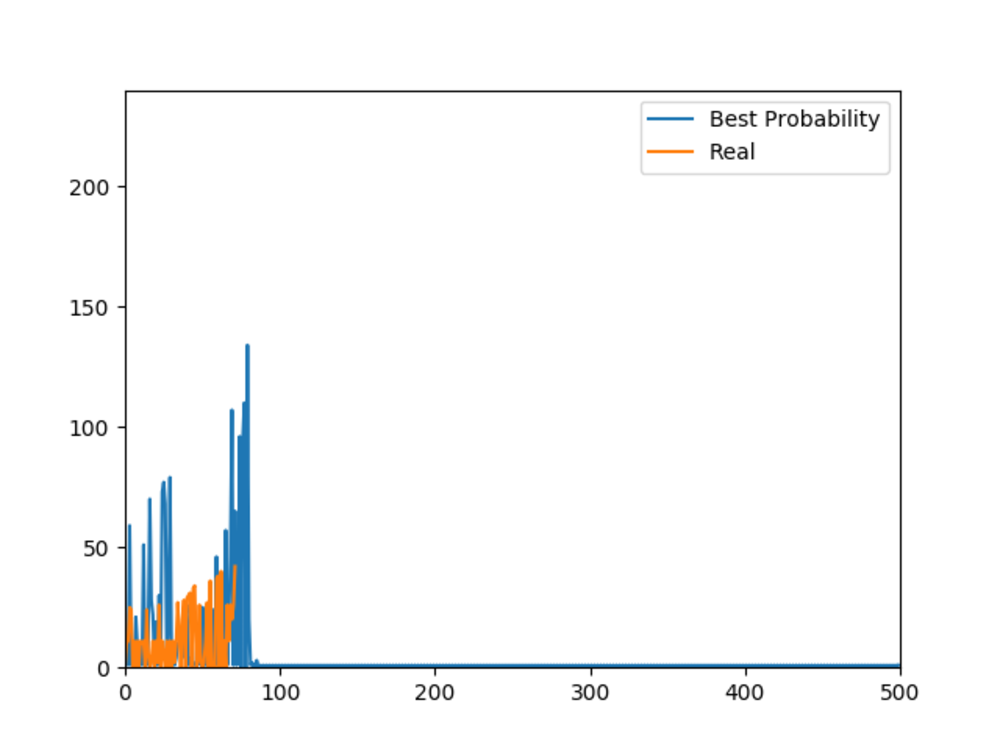
\includegraphics[width=1\textwidth]{Generate/H5N50T5/user109Normal2.pdf}}
\textbf{\caption{Best Probability Generator with 500 steps generated}
\label{fig:genN4}}
\end{minipage}
\hfill
\begin{minipage}{0.48\textwidth}
\centering
\raisebox{-\height}{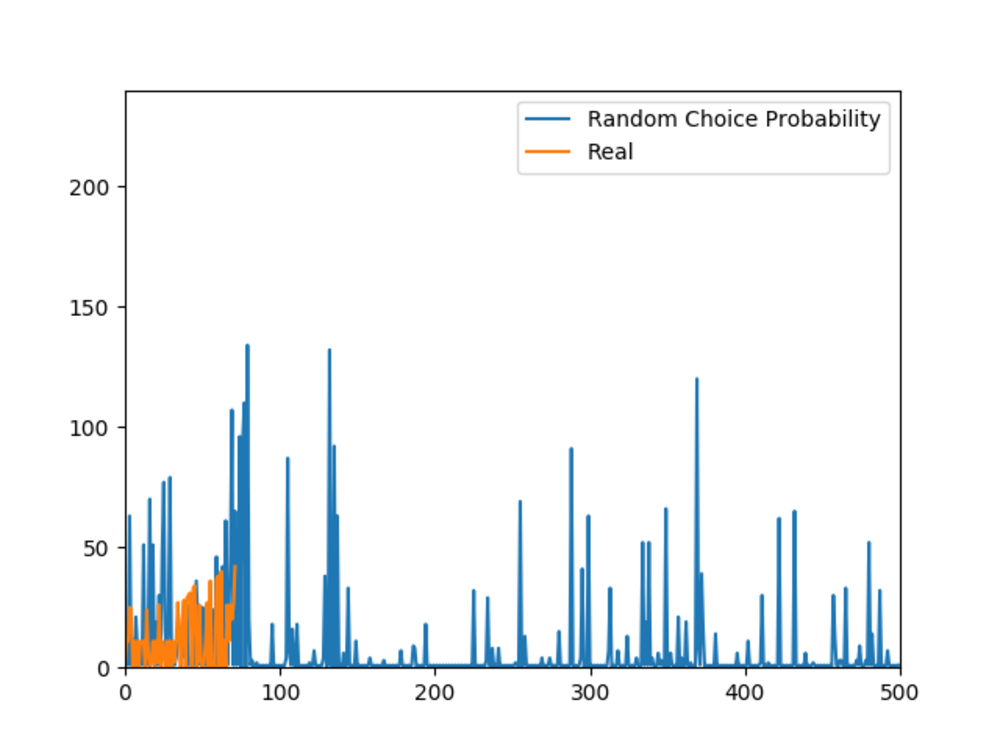
\includegraphics[width=1\textwidth]{Generate/H5N50T5/user109Choice2.pdf}}
\textbf{\caption{Random Choice Probability Generator with 500 steps generated}
\label{fig:genC4}}
\end{minipage}
\end{figure}

\begin{table}[t!]
\centering
\begin{tabular}{l|r|r|r|r|}
\cline{2-5}
\textbf{}                       & \multicolumn{1}{c|}{\textbf{Random}} & \multicolumn{1}{c|}{\textbf{Best Probability}} & \multicolumn{1}{c|}{\textbf{Random Choice Probability}} & \multicolumn{1}{c|}{\textbf{Real}} \\ \hline
\multicolumn{1}{|l|}{Mean}      & 118.547                              & 2.505                                          & 7.376                                                   & 17.009                             \\ \hline
\multicolumn{1}{|l|}{Median}    & 118.77                               & 1.87                                           & 2.4                                                     & 8.3                                \\ \hline
\multicolumn{1}{|l|}{Maximum}   & 236.82                               & 50.807                                         & 127.333                                                 & 82.827                             \\ \hline
\multicolumn{1}{|l|}{Minimum}   & 0.12                                 & 0.2                                            & 0.053                                                   & 0.413                              \\ \hline
\multicolumn{1}{|l|}{Unique}    & 209.287                              & 10.04                                          & 43.267                                                  & 30.393                             \\ \hline
\multicolumn{1}{|l|}{Std}       & 68.635                               & 5.044                                          & 16.55                                                   & 22.919                             \\ \hline
\multicolumn{1}{|l|}{Skew}      & -0.001                               & 7.189                                          & 4.07                                                    & 1.737                              \\ \hline
\multicolumn{1}{|l|}{Amplitude} & 118.35                               & 25.303                                         & 63.64                                                   & 41.207                             \\ \hline
\multicolumn{1}{|l|}{Max slope} & 228.013                              & 48.14                                          & 125.867                                                 & 80.667                             \\ \hline
\end{tabular}
\centering
\textbf{\caption{Some measures extracted from the synthetical trajectories of the different generators (500 steps)}
\label{table:generators2}}
\end{table}

With these results, we can clearly consolidate the first thought that a generator based only on random is really not recommended in synthetic trajectories. Indeed only bad results will be obtained in the applications mentioned before as traffic management. All results also consolidated the thought that some memory of past positions can help for better capture behavior of people. The results on generators based on the RNN-LSTM model show us that we clearly obtain better results than random or just taking best occurrences.

It shows also that taking only purely the higher probability given by the RNN-LSTM model for the next position is not perfect, particularly when we try to generate large steps. It can give us the problem of falling in a particular cycle without a lot of variances, so a monotone behavior without the little magic of the human kind for the change. The results conclude also that combining just a little bit of random in the generator can really help to produce a more human-like path. 

It is really hard to say which one of the two generators has to be used: based only on best probability or combined with some random. It depends on the trajectories needed and on what kind of purpose and application. For instance, if we need to predict only a little projection of the movement of one user as its three next steps, it will be better to use only the Best Probability Generator. In contrary, if we need to simulate a large number of human movements, for example in traffic simulation, it will be clearly better to use the Random Choice Probability Generator.


%----------------------------------------------------------------------------------------
% Discussion
%----------------------------------------------------------------------------------------
\newpage
\section{Discussion}
%overwiew
Since decades the increasing movements of people have profoundly changed tendencies. New needs, new opportunities and also new problems have appeared. Moreover, the globalization of technologies has accentuated these effects. As a result, a lot of applications linked to these movements exist or could be created. These different applications need very large datasets about mobility and at the same time, it is very difficult to obtain data, mainly due to privacy \cite{kulkarni}. It is why it is interesting to generate the data needed for mobility in order to need no more real one or at least less. As we viewed, it is difficult to capture the real behavior of humans in order to generate realistic trajectories, as shown by some existing work on bird migration \cite{technitis} or city network \cite{jiang2009characterizing}. Indeed most of them work only with a stochastic process without really capturing global human mobility behavior. That is why we have looked for some models capable of capturing the real behavior of people such as machine learning techniques. Moreover, in our context, past positions influence significantly the trajectories. This is the reason why we focused on a model capable of learning long-term dependencies and RNN models seem to be appropriate \cite{kulkarni} for this task.

%prediction
During the prediction part of the project, the need to understand the context and its characteristics appeared. For instance, we saw already the importance of timesteps in the context of mobility. Moreover, we saw that we could nearly always adapt our models to the task needed. For instance, even if the other models than the RNN have no parameter such as timestep, we transformed the size of their input to fill the gap. Indeed by this way, we simulated timesteps of the RNN-LSTM model and so they could capture the human movement behaviors on their previous movements. We saw also that even if basic models seemed to try to capture some behaviors, it would have been very difficult to improve their performance given their lack of evolving parameters. Fortunately, the RNN-LSTM is adapted for predicting mobility trajectories, especially because of its powerful flexibility and ability to capture long-term dependencies. 

%optimize
Furthermore during the optimization using some timesteps clearly improved the results to finally obtain something that really seemed to integrate the behavior of users. The RNN-LSTM model responds very well when trying to figure out what is the optimal set of parameters. It confirms that a larger model with more neurons and hidden layers than a simple one tends to recognize more patterns and captures them. Until a certain limit, we see that increasing the size of the models increases their performances, but reaching this limit no major good effects occur. Sometimes it even decreases the performance and increases also the training time. We see that smaller models have worse results than our best one. We can not withdraw the possibility that with a longer training time, the larger models may have better results, but this is unlikely. With our setting, we are confident that we have found the best hyperparameters, especially when looking to the Mean, Median, Standard Deviation, and P-value.

%generator
The results from the generation stage confirm that generating a path based only on random is not imaginable for mobility trajectories. Therefore, using something to integrate the real pattern of the human mobility is the key, as is confirmed by the results of the RNN-LSTM model. Even if the model is not yet sufficient to generate perfect synthetic mobility trajectories, the Random Choice Probability Generator at least confirms that it can be possible. In further works, it would be interesting to continue improving the model, using some other features (time, delta time between movements, or others) or test it on other datasets. Moreover, we could also take a look at other models, even more complex. Indeed the Generative Adversarial Networks (GANs) could show promising results. This is a model composed of two submodels. Indeed a GANs puts two models in competitions: one that generates fake data and the other one that attempts to predict if the data given is real or false. It could be possible to use it in our case to generate synthetic mobility trajectories and even to integrate an RNN-LSTM in it. 


%----------------------------------------------------------------------------------------
% Conclusion
%----------------------------------------------------------------------------------------
\newpage
\section{Conclusion}%3 paragraph
%overwiew
The high level of movements of people has created new tendencies, new needs, new problems and new opportunities. A lot of applications linked to these movements exist or could be created. Unfortunately, these applications need large datasets about mobility and privacy restriction of user data is strongly binding. It is why it is interesting to generate the data needed for mobility in order to need no more real one or at least less. Some existing works have tried to generate trajectories. Most of them work only with a stochastic process without really capturing global human mobility behavior. That is why we have focused on machine learning techniques and the idea of memory of past positions to capture human mobility behavior. This is the reason why we focused on a model capable of learning long-term dependencies and RNN models proved to be appropriate for this task.
After having compared four different models, our hypothesis is confirmed. The idea of keeping some past information about the trajectories to perform better is clearly confirmed. Even with basic models as Linear Regression model or Logistic Regression model the use of some past information provides better results. Moreover, according to some experiences performed we found an optimal RNN-LSTM for predictions with 5 timesteps, 5 hidden layers with 50 neurons each. Furthermore, we created and tested three different generators for transitions between points of interest. The first one is based exclusively on random. The second one is based only on best probability prediction from our RNN-LSTM model. The last one uses a random choice process on the prediction from our RNN-LSTM. This last generator procures better results by generating more realistic trajectories, especially when we try to generate numerous steps. Indeed its trajectories nearly never fall in redundant cycles of the same positions. Moreover, some measures extracted from it confirm its superiority, especially about  Mean, Median, Unique, Standard Deviation, and Amplitude.
The present master thesis proves us that the machine can capture and understand some human behavior in a context of geospatial trajectories. Even if the present work uses only a simplification of the problem by using only sequences of areas, we can see the efficacy of RNN-LSTM. It would be really interesting to go further in the context and try, for example, to add and test the impact of more features such as time, delta time, longitude and latitude. Moreover, we could also take a look at a model even more complex as Generative Adversarial Networks (GANs) which could be assembled with our RNN-LSTM. Ultimately we have proved that RNN-LSTM can be applied to generate realistic trajectories. Further development is necessary in order to create a generator usable for real applications in the fields of synthetic geospatial trajectories.


%----------------------------------------------------------------------------------------
\newpage

\bibliographystyle{plain}
\bibliography{Biblio}

\newpage
\listoffigures
 \newpage
\listoftables

%----------------------------------------------------------------------------------------
\newpage
\clearpage
%\appendix
%\section{Software, libraries and tools}
\appendix
\section{\\Software, libraries and tools used}
IntelliJ IDEA 2017.2.3
\\Tensorflow 1.3.0
\\Cesium 0.9.4
\\Python 3.5.4
\\Jupyter Notebook 5.3.0
\\Github \footnote{Codes and documents of the project can be found by following the link \url{https://github.com/YPatschke/MachineLearning}}



\end{document}
